\chapter{Quellen und Methoden}\label{sec:Quellen}
\begin{multicols}{2}
\raggedcolumns
\noindent Das im Rahmen dieser Arbeit bearbeitete Quellenmaterial umfasst 10\,519 Fundstücke von 122 individuellen Fundplätzen in einem 500\,$\times$\,700\,km großen Arbeitsgebiet (Kap.~\ref{sec:Arbeitsgebiet}). Das Material stammt zu einem großen Teil aus 143 individuellen Oberflächenabsammlungen.\footnote{Während an allen Fundstellen mindestens die moderne Dorffläche nach Funden wie Befunden abgesucht wurde, existieren von einigen Plätzen Komplexe aus zusätzlichen, spezifischen Bereichen (siehe Katalog B).} Eine belastbare Quellenbasis bildeten 13 ausgegrabene sowie sechs weitere, zwar als Befunde erkannte, aber nicht systematisch untersuchte Komplexe (Tab.~\ref{TabBefundeUntersucht}). Da keine exakten geografischen Koordinaten der Fundstellen bekannt waren, mussten diese nachträglich ermittelt werden.\footnote{Die Fundstellen wurden während der Befahrung der Flüsse in Flussatlanten, welche von der staatlichen, damals za{\"i}rischen Transport- und Schifffahrtsbehörde ONATRA (\textit{Office national des Transports}) stammten, verzeichnet. Die Erhebung der Koordinaten erfolgte durch Abgleich dieser um entsprechende Notizen ergänzten Flussatlanten mit GoogleEarth-Satellitendaten. Diese Vorgehensweise bedingt eine gewisse Unschärfe der ermittelten Positionen, da es von Fall zu Fall kleinere Unterschiede im Kartenmaterial gab. Die Positionen der Fundstellen innerhalb der Ortschaften ließ sich regelhaft nicht mehr präzise rekonstruieren. Die in GoogleEarth ermittelten Koordinaten für die Fundstellen wurden in Dezimalgrade umgerechnet und als Längen- sowie Breitenangabe aufgenommen (Anlage 1.B).} Die Vergabe von Katalognummern, im weiteren als \enquote{Fpl.} abgekürzt, schließt an den 185 Fundstellen umfassenden Katalog von \textcite[542\,f. Karte 1]{Wotzka.1995} an.

Die Aktenlage umfasste neben der ursprünglichen Dokumentation\footnote{Aufgrund des zeitlichen Abstandes zwischen den Feldarbeiten des \textit{River Reconnaissance Project} in den 1980er Jahren und der aktuellen Aufarbeitung konnten offene Fragen an die ursprüngliche Dokumentation nicht immer zufriedenstellend geklärt werden. Als zentrales Problem erwies sich das Fehlen der schriftlichen Felddokumentation von Célestin Kanimba Misago, dem damaligen Mitarbeiter der \textit{Musées Nationaux du Zaïre} (heute \textit{Institut des Musées Nationaux du Congo}) in Kinshasa und Kooperationspartner. Während die Feldbücher der übrigen Teilnehmer der Reisen von 1985 und 1987 im Original wie in Kopie vorlagen, konnten jene von Kanimba Misago nicht aufgefunden werden. Während der Kampagne von 1987 hatte Kanimba Misago die Komplexe BBS~87/1 (Kat.-Nr.~6) in Bobusa am unteren \mbox{Sangha} (Fpl.~239) und PIK~87/3 (Kat.-Nr.~10) in Pikunda am mittleren \mbox{Sangha} (Fpl.~255) ausgegraben. Der Metallurgie-Befund PIK~87/3, welcher nach Ausweis der vorliegenden Radiokohlenstoffdatierung in das 11.--13.~Jh. n.~Chr. (Abb.~\ref{fig:PIK87_Datierungen}) datiert und damit einer der ältesten Belege für einen flachen, offenen Ofen mit Schlackeabfluss in der Region darstellt, konnte ausschließlich auf einer nur bedingt systematischen fotografischen Dokumentation sowie einer Kurzbeschreibung durch \textsc{Kanimba Misago} aus dem Jahr 1995 beschrieben werden (Details siehe Kat.-Nr.~10), was bei der Bedeutung des Befundes bedauerlich ist.}, die im Gelände angefertigt wurde, auch eine Reihe von internen Berichten und Teile unveröffentlichter Manuskripte. Wo diese für die Aufarbeitung des Materials herangezogen wurden, sind sie entsprechend als Quelle im Text ausgewiesen. Die in dieser Arbeit durchgeführten Analysen gründen sich in allen Fällen auf den eigenen Beobachtungen des Autors am Fundmaterial sowie der Auswertung der im Gelände angefertigten Dokumentation (Katalog~A).

\section{Surveys, Grabungen und Befunde}\label{sec:GrabungenBefunde}

\subsection{Grubenbefunde}

In die Auswertung flossen 13 Grabungsbefunde von fünf verschiedenen Fundstellen ein sowie sechs Komplexe, die zwar einen klaren Befundcharakter aufweisen, aber nicht systematisch ergraben wurden (Tab.~\ref{TabBefundeUntersucht}, Katalog A). Zu letzterer Gruppe werden zum Beispiel die Komplexe MLB~85/103 (Kat.-Nr.~5) und LKW~87/186 (Kat.-Nr.~19) gerechnet, die zwar eindeutig als Gruben angesprochen werden können, jedoch nicht ausgegraben wurden. Da sich diese Beobachtungen aber aufgrund ihrer Geschlossenheit grundsätzlich von den ebenfalls in die Gesamtauswertung eingeflossenen Surveyfunden (Katalog B) unterscheiden, werden sie gemeinsam mit den Grabungsbefunde besprochen.

\begin{table*}[!t]
\centering
%\resizebox{\textwidth}{!}{%
{\footnotesize
\begin{sftabular}{@{}lllll@{}}
\toprule
\textbf{Fundstelle} & \textbf{Gruben} & \begin{tabular}[c]{@{}l@{}}\textbf{Metallurgie-}\\ \textbf{befunde} \end{tabular} & \textbf{Gräber} & \begin{tabular}[c]{@{}l@{}}\textbf{Schichten-}\\ \textbf{Abfolge} \end{tabular} \\
\midrule
\begin{tabular}[c]{@{}l@{}}\textbf{Maluba}\\(Fpl.~230)\end{tabular} & \begin{tabular}[c]{@{}l@{}}MLB 85/1-3-1\\ MLB 85/1-3-2\\ (MLB 85/2)\\ (MLB 85/103)\end{tabular} & & MLB 85/1-4-3 & \\ %\hdashline
\begin{tabular}[c]{@{}l@{}}\textbf{Bobusa}\\(Fpl.~239)\end{tabular} & & & & \begin{tabular}[c]{@{}l@{}}BBS 87/1\\ BBS 87/2\end{tabular} \\[3ex] %\hdashline
\begin{tabular}[c]{@{}l@{}}\textbf{Pikunda}\\(Fpl.~255)\end{tabular} & \begin{tabular}[c]{@{}l@{}}PIK~87/1\\ PIK~87/2\end{tabular} & PIK~87/3 & & \\[3ex] %\hdashline
\begin{tabular}[c]{@{}l@{}}\textbf{Ngombe}\\(Fpl.~252)\end{tabular} & (NGO~87/102) & & & \\[3ex] %\hdashline
\begin{tabular}[c]{@{}l@{}}\textbf{Mitula}\\(Fpl.~251)\end{tabular} & (MIT~87/103) & & & \\[3ex] %\hdashline
\begin{tabular}[c]{@{}l@{}}\textbf{Mobaka}\\(Fpl.~246)\end{tabular} & (MKA~87/102) & & & \\[3ex] %\hdashline
\begin{tabular}[c]{@{}l@{}}\textbf{Boleko}\\(Fpl.~285)\end{tabular} & & & BLK 87/1 & \\[3ex] %\hdashline
\begin{tabular}[c]{@{}l@{}}\textbf{Likwala Fluss-}\\ \textbf{Kilometer~186}\\(Fpl.~291)\end{tabular} & (LKW~87/186-1) & & & \\[3ex] %\hdashline
\begin{tabular}[c]{@{}l@{}}\textbf{Munda}\\(Fpl.~304)\end{tabular} & \begin{tabular}[c]{@{}l@{}}MUN~87/2-1-1 A \\ MUN~87/2-1-3\end{tabular} & \begin{tabular}[c]{@{}l@{}}MUN~87/1 \\ MUN~87/2-1-1 B/C \\ MUN~87/3\end{tabular} & & \\
\bottomrule
\end{sftabular}}
%}
\caption{Ausgegrabene Befunde: Übersicht über die untersuchten Befunde im Arbeitsgebiet aufgeteilt nach Befundkategorien. Die in Klammern stehenden Komplexe wurden nicht systematisch ausgegraben, aber als Befunde erkannt. Die Sortierung der Liste orientiert sich an der Abfolge, in der die Befunde untersucht wurden.}
\label{TabBefundeUntersucht}
\end{table*}

Im Jahr 1985 wurden bei der Befahrung der Flüsse \mbox{Ubangi} und Lua lediglich in Maluba am Lua (Fpl.~230, Kat.-Nr.~1--5) Grabungen durchgeführt. Von den insgesamt vier dort beobachteten Gruben wurden nur zwei vollständig untersucht und dokumentiert (Kat.-Nr.~1--2). Die ursprüngliche Verfüllung einer weiteren Grube (Kat.-Nr.~4) stürzte während der Grabung ein. Daher wurde der Befund nicht mehr weiter untersucht. Es wurden auch keine Funde dieses Befundes geborgen beziehungsweise zur Auswertung lagen keine Funde aus dieser Grube mehr vor. Eine vierte Grube (Kat.-Nr.~5) ist zwar als solche zu erkennen gewesen, es wurde aber lediglich eine geringe Menge keramischen Fundgutes entnommen und keine Grabung durchgeführt. Während der Kampagne von 1987 im nördlichen Teil der Republik Kongo, entlang der Flüsse \mbox{Sangha}, \mbox{Ngoko} und Liwkala-aux-Herbes sowie eines kurzen Abschnitts des Kongo, wurden zehn Befunde an vier verschiedenen Fundstellen untersucht. In Pikunda am mittleren \mbox{Sangha} (Fpl.~255) wurden an zwei benachbarten Grabungsstellen insgesamt drei Gruben (Kat.-Nr.~8--9) erfasst. In Munda am \mbox{Likwala}-\mbox{aux}-\mbox{Herbes} (Fpl.~304) fanden die umfangreichsten Ausgrabungen des \textit{River Reconnaissance Project} im Arbeitsgebiet statt. Innerhalb eines eng begrenzten Areals wurden vier Komplexe näher untersucht, die drei Gruben sowie drei Verhüttungsbefunde erbrachten. Die Grabungen MUN~87/1 (Kat.-Nr.~15) sowie MUN~87/2--1--1 (Kat.-Nr.~16) ergaben jeweils eine Grube sowie einen Verhüttungsbefund, während es sich bei Befund MUN~87/2--1--3 (Kat.-Nr.~17) um eine weitere Grube handelt.

Für das \mbox{Sangha}- und Likwala-aux-Herbes-Gebiet lassen sich auf Basis der ausgegrabenen Befunde in Pikunda (Fpl.~255) und Munda (Fpl.~304) Grundlagen der chronologischen Sequenz erarbeiten (siehe Kap.~\ref{sec:SequenzLikwala}--\ref{sec:SequenzSanghaNgoko}). Die Grabungen in Maluba am Lua (Fpl.~230) decken nur eine der belegten keramischen Stilgruppen ab und ermöglichen kaum weiterführende Aussagen zum Ablauf der Besiedlung im \mbox{Ubangi}- und Lua-Gebiet. Zwar liefern die Funde aus ausgegrabenen Kontexten oder eindeutig ansprechbaren Befunden die beste Datenlage, jedoch spiegeln sie nur sehr begrenzte Nutzungsphasen innerhalb der jeweiligen Fundstelle wider.

In Zentralafrika sind Grundbefunde die am häufigsten dokumentierte Befundkategorie und auch im Arbeitsgebiet wurden vor allem Gruben untersucht. Die Frage nach der Bedeutung dieser Befunde -- ihre Nutzung und Funktion in der Vergangenheit -- ist Gegenstand einer anhaltenden Diskussion \parencite[siehe][197--199]{Meister.2008b}. Während Merkmale wie die häufig in den Befunden beobachtete fragmentierte Gefäßkeramik sowie botanische Reste vordergründig eine profane Nutzung nahelegen, deuten andere Eigenschaften andere Verwendungen an. Der bislang ambitionierteste Interpretationsansatz stammt von \textcite{Wotzka.1993} und gründet auf die Feldarbeit des \textit{River Reconnaissance Project} sowie einem detaillierten Survey ethnologischer Literaturbelege. Die von Wotzka bearbeiteten 34 Grubenbefunde des Inneren Kongobeckens und die dabei beobachteten Deponierungen von Gefäßkeramik in ihnen bildeten die Grundlage für seine Auseinandersetzung mit der Frage nach der Funktion von Keramikdeponierungen in Gruben im zentralafrikanischen Regenwald. \textsc{Wotzka} (ebd. 262\,f. Tab.~1) stellte die an den Grubenbefunden beobachteten Merkmale zusammen und beschrieb sie im Sinne einer polythetischen, sich aus überschneidenden Typen zusammensetzenden Gruppe \parencite[siehe][37\,f. mit Abb.~3]{Clark.1968}. Aus archäologischer Perspektive kann er deutlich machen, dass es sich bei den von ihm untersuchten Befunden nicht um reine \mbox{Abfall-,} Vorrats-, Lehm- oder Lateritentnahmegruben handelt \parencite[264]{Wotzka.1993}. In der von ihm gesichteten ethnographischen Literatur berücksichtigte er auch an Gefäßkeramik aus Gruben beobachtbare Modifikationen oder intentionellen Zerstörungen von Böden oder Appliken (ebd.~262\,f. Tab.~1 Merkmale 6, 13 und 15). In seiner abschließenden Bewertung steht für \textsc{Wotzka} (ebd. 272) die \enquote{Erkenntnis, dass es zahlreiche in rezenter und subrezenter Zeit beobachtete Belege für rituelle Zerstörung von Keramik und anderen Sachgütern gibt, die in einem allgemeinem Zusammenhang mit dem Totenkult stehen}.\footnote{Erste geochemische Untersuchungen von Grubensedimenten aus Fundstellen in Südkamerun offenbarten eine Anreicherung von Phosphat im Bereich der Grubensohlen \parencites[722--724]{MbidaMindzie.19951996}{MbidaMindzie.1998}[147--150; 151--155]{Eggert.2016}. Während \textcite[209]{MbidaMindzie.1998} die auffällige Phosphatanreicherung, die in drei Gruben der Fundstelle Nkang beobachtet wurde, mit anthropogenen Faktoren in Verbindung bringt, weisen \textcite[151--155]{Eggert.2016} auf die Nichtberücksichtigung einer durch die niedrigen ph-Werte möglichen natürlichen Akkumulation hin. Im Zuge der vorliegenden Untersuchung wurde die Fragmentierung der in den Grubenbefunden des Arbeitsgebietes angetroffenen Gefäßkeramik dezidiert aufgenommen (siehe Abb.~\ref{fig:Fragmenierung_MLB85-131}, \ref{fig:Fragmenierung_MLB85-132}, \ref{fig:Fragmenierung_BBS87-1}, \ref{fig:Fragmenierung_BBS87-2}, \ref{fig:PIK87-1_Fragmentierung}, \ref{fig:BLK87-1_Keramik_Fragm}, \ref{fig:MUN87-1_Fragmentierung}, \ref{fig:MUN87-211_Fragmentierung}, \ref{fig:MUN87-213_Fragmentierung}). Während diese Verteilungen zwischen den verschiedenen Formen von Gruben und generell zwischen den Befundkategorien deutlich voneinander abwichen, steht eine spezifische Diskussion der daraus abzuleitenden Schlüsse noch aus.\label{ftn:GeochemieGruben}} Eine universelle Ansprache der Nutzung und Funktion von Gruben in Zentralafrika ergibt sich auch durch die Studie Wotzkas nicht, jedoch erweitert sie den Interpretationsansatz über allzu simple, profane Nutzungsmuster hinaus um eben jene sozialen Komponenten, die Gruben und vor allem die charakteristischen Deponierung von Gefäßkeramik als Teil des Alltags der prähistorischen Gesellschaften Zentralafrikas interpretierbar machen. Weiterhin muss jeder Befund individuell angesprochen und auf seine Genese hin untersucht werden.\footnote{Der Wandel von Nutzungsmustern über die Dauer des Bestehens eines Befundes lässt sich in geradezu exemplarischer Weise am Befund MUN~87/2-1-1 (Kat.-Nr.~16) in Munda am oberen \mbox{Likwala}-\mbox{aux}-\mbox{Herbes} (Fpl.~304) ablesen.}


\subsection{Sonstige Befunde}

Neben den Gruben zählen zu den archäologisch untersuchten Befunden im Arbeitsgebiet noch vier weitere Strukturen, die mit Eisenerzverhüttung in der Region in Zusammenhang gebracht werden können (Tab.~\ref{TabBefundeUntersucht}). Einer dieser Befunde wurde in Pikunda am \mbox{Sangha}, zusätzlich zu den genannten Gruben, als dritte Grabungsstelle erfasst (Kat.-Nr.~10). Die drei übrigen Befunde dieser Kategorie wurden ebenfalls 1987 bei den Ausgrabungen in Munda am \mbox{Likwala}-\mbox{aux}-\mbox{Herbes} untersucht. Neben den in den beiden Grabungsstellen MUN~87/1 (Kat.-Nr.~15) sowie MUN~87/2-1-1 (Kat.-Nr.~16) erfassten Verhüttungsstrukturen wurde in unmittelbarer Nähe ein weiterer Ofenbefund beobachtet und unter der Befundnummer MUN~87/3 (Kat.-Nr.~18) untersucht.

Zusätzlich zu den genannten Verhüttungsbefunden wurden zwei Bestattungen erfasst. Bei der Grabung im Jahr 1985 in Maluba am Lua (Fpl.~230) wurde zwischen den beiden ausgegrabenen Gruben (Kat.-Nr.~1--2) eine in einer kleinen Eingrabung angelegte Sekundärbestattung (Kat.-Nr.~3) erfasst und dokumentiert. Ein subrezentes Körpergrab (Kat.-Nr.~14) wurde 1987 in Boleko am \mbox{Likwala}-\mbox{aux}-\mbox{Herbes} (Fpl.~285) archäologisch untersucht.

Zwei zur Erfassung der jeweiligen Schichtabfolgen angelegte Sondageschnitte in Bobusa an der Mündung des \mbox{Sangha} (Fpl.~239) wurden ausgehend von bestehenden Bodeneingriffen angelegt. Sie waren jeweils nur 1\,m\textsuperscript{2} groß und reichten nur bis in etwa 1\,m Tiefe (Kat.-Nr.~6--7).


\subsection{Surveys}

Etwa zwei Drittel der untersuchten Funde stammen von Oberflächenabsammlungen. Zusammengenommen konnten 143 separate Komplexe von 118 Fundstellen herangezogen werden. Da die ausgegrabenen Befunde nur einen ungenügenden Einblick in die chronologischen Relationen zwischen den keramischen Stilgruppen boten und somit eine Rekonstruktion des Besiedlungsganges auf Basis dieser Daten nicht möglich war, musste dem von der Oberfläche der Dörfer abgesammelten Material verstärkt Beachtung geschenkt werden. Die Inventare aus Oberflächenabsammlungen setzen sich im Mittel aus jeweils gerade einmal 40 Fundstücken zusammen. Während die umfangreichsten Komplexe aus bis zu 289 Stücken bestehen, setzt sich die Hälfte aller Oberflächenabsammlungen aus weniger als 22 Fundobjekten zusammen. Neben den grundsätzlichen Schwierigkeiten im Umgang mit Funden aus Oberflächensurveys illustrieren die genannten statistischen Kennzahlen die Probleme bei der quantitativen Auswertung der entsprechenden Komplexe.

Die interne Zusammensetzung von Komplexen aus Oberflächensurveys ist grundsätzlich vielfältigen Parametern unterworfen.\footnote{Die Zusammensetzung eines Komplexes aus einem Oberflächensurvey ist nur zum Teil durch die archäologische sowie geomorphologische Situation an der Fundstelle bestimmt. In den hier zur Untersuchung vorliegenden Funden aus Dörfern im Zentralafrikanischen Regenwald ist aufgrund der gängigen Praxis des Fegens der Dorffläche zur Reinhaltung vor Bewuchs und Kleintieren mit einer großen Verlagerung von Objekten innerhalb der Fundstelle zu rechnen \parencite[355 Anm.~1]{Wotzka.1995}. Darüber hinaus spielen aber auch Faktoren eine Rolle, die mit dem Survey selbst zu tun haben, wie die Witterung, die Nutzung spezifischer Bereiche eines Dorfes zum Zeitpunkt des Surveys und auch die Erfahrung des Sammelnden.} Indizien für eine mögliche Vermischung von Funden ergaben sich im Zuge der Auswertung der Survey-Inventare von zwei im Gelände unterschiedenen Bereichen einer Fundstelle. Im Fall von zwei anderen Inventaren wurde eine Vermischung der Funde bereits 1990 festgestellt.\footnote{Aus Bobusa am unteren \mbox{Sangha} (Fpl.~239) liegen zwei direkt anpassende Scherben eines Reiseherdes vor (siehe Kap.~\ref{sec:Reiseherde}). Während ein Stück im Dorf (BBS~87/101:10) gefunden wurde, stammt eine weiteres, direkt anpassendes Fragment aus der als \textit{elali} (siehe Anm.~\ref{ftn:elali}) bezeichneten Dorfwüstung (BBS~87/102:81). Nach den Angaben im Feldbuch von Manfred Eggerts lag das \textit{elali} etwa 7 Weg-Minuten vom Dorf entfernt. Auf Basis der vorliegenden Unterlagen kann eine simple Verwechslung der Nummerierung bei der Beschriftung der Stücke im Anschluss an die Feldkampagne von 1987 nicht ausgeschlossen werden. Inwieweit eine mögliche Verlagerung der Funde auf natürlichem oder artifiziellem Wege bestehen kann, muss offenbleiben. Das Material des Komplexes NGO~87/101 aus Ngombe am \mbox{Sangha} (Fpl.~252) wurde zu einem nur grob eingrenzbaren Zeitpunkt mit jenem des Komplexes NGL~87/101 aus Ngombe am \mbox{Likwala}-\mbox{aux}-\mbox{Herbes} (Fpl.~283) vermischt. Allen Funden des Komplexes NGO~87/101 wurde die Kennung NGL~87/101 gegeben. Erkannt wurde dieser Umstand erst 1990 von Eggert, als ihm bei einer Durchsicht der Funde der Kampagne von 1987 auffiel, dass \textit{offiziell} keine Funde mit der Kennung NGO 87/101 vorliegen. Im Fall der Scherben aus den beiden Fundstellen muss die Vermischung bereits sehr zeitig, möglicherweise bereits im Feld, bei der Vorbereitung des Exports der Funde oder kurz danach stattgefunden haben. In den verfügbaren Packlisten waren bereits nur die beiden Komplexe NGL~87/101 und NGO~87/102 und kein Komplex NGO~87/101 verzeichnet. Ein entsprechender Komplex ist jedoch eindeutig im Feldbuch Eggerts sowie der Kartei der Fundstellenkürzel mit der Beschreibung \enquote{Dorf allgemein} ausgewiesen. Im Zuge der Aufarbeitung der Funde ergaben sich nur wenige stichhaltige Indizien, die eine Trennung des mit NGL~87/101 beschrifteten Materials, insgesamt 112 Scherben, auf zwei Komplexe ermöglichten. Auffällig ist das Auftreten von rouletteverzierter Keramik, die an Fundstellen entlang des Likwala-aux-Hebers kaum beobachtet wurde (siehe Kap.~\ref{sec:SequenzLikwala}), am \mbox{Sangha} jedoch durchaus vertreten ist (siehe Kap.~\ref{sec:SequenzSanghaNgoko}). Beruhend auf den Inventaren der jeweils benachbarten Fundstellen konnte unter Vorbehalten das jeweilige Ensemble der Stilgruppen an den beiden Fundplätzen rekonstruiert werden (siehe Tab.~\ref{tab:LikwalaSequenz}, \ref{tab:SanghaNgokoSequenz}).\label{ftn:Vermischungen}}

\section{Funde}

Die umfangreichste Fundgattung innerhalb des untersuchten Materials bildet die Gefäßkeramik (Tab.~\ref{tab:Funde_Uebersicht}). Die insgesamt 8469 Gefäßeinheiten und Scherben machen 80\,\% des gesamten Fundgutes aus. Unter den restlichen, nichtkeramischen Funden nehmen Metallurgieüberreste, vor allem Schlacken mit 1321 Stücken beziehungsweise knapp 40\,kg eine hervorzuhebende Stellung ein. Die weiteren Fundkategorien sind häufig nur durch wenige Stücke vertreten.

\begin{figure*}[tb]
\noindent\begin{minipage}[b]{\columnwidth}
	\includegraphics[width=\columnwidth]{fig/2-2_FundeGewicht_FlussKM.pdf}
	\captionof{figure}{Funde: Vergleich des Fundaufkommens (hell) mit Bezug auf die Länge des befahrenen Flussabschnitts (dunkel).\label{fig:FundGewVSFlussKM}}
\end{minipage}\hfill
\noindent\begin{minipage}[b]{\columnwidth}
{\footnotesize \begin{sftabular}{@{}p{.325\columnwidth}R{.125\columnwidth}R{.075\columnwidth}R{.175\columnwidth}R{.075\columnwidth}@{}}
		\toprule
		\textbf{Fundkategorie} &  \textbf{Anzahl} &     \textbf{\%} &  \textbf{Gew. (kg)} &     \textbf{\%} \\
		\midrule
		Gefäßkeramik &    8469 &   80,5 &        363,34 &   78,3 \\
		Schlacke &    1321 &   12,6 &         39,73 &    8,6 \\
		gebrannter Lehm &     187 &    1,8 &          6,25 &    1,3 \\
		Ofenwand &     182 &    1,7 &         19,88 &    4,3 \\
		keram. Sonderform &     117 &    1,1 &         11,19 &    2,4 \\
		Tuyere &      94 &    0,9 &          6,81 &    1,5 \\
		Stein &      76 &    0,7 &          7,23 &    1,6 \\
		Knochen &      29 &    0,3 &          5,93 &    1,3 \\
		Eisen &      13 &    0,1 &          0,53 &    0,1 \\
		Laterit &      11 &    0,1 &          0,08 &    0,0 \\
		Glas &       6 &    0,1 &          0,01 &    0,0 \\
		Metall &       8 &    0,1 &          0,38 &    0,1 \\
		Botanik &       2 &    0,1 &             - &      - \\ 
		Sonstige &       5 &    0,1 &          2,52 &    0,5 \\ \bottomrule			\multicolumn{1}{r}{\textbf{$\sum$}} &   10519 &  100 &        463,88 &  100 \\
		\bottomrule
	\end{sftabular}
}
\captionof{table}{Funde: Übersicht der in die Auswertung eingeflossenen Fundkategorien und ihrer Anteile.\label{tab:Funde_Uebersicht}}
\end{minipage}
\end{figure*}

Die Funde sind, obschon der Geländearbeit innerhalb beider Kampagnen die gleiche Surveystrategie zugrunde lag, nicht gleichmäßig im Arbeitsgebiet verteilt. Während einige Regionen sehr gut repräsentiert sind, liegen aus anderen Räumen nur vergleichsweise wenige Funde vor. Besonders deutlich wird dies bei einer Gegenüberstellung des Fundaufkommens von den drei größten, befahrenen Flüssen: \mbox{Ubangi}, \mbox{Sangha} und \mbox{Likwala}-\mbox{aux}-\mbox{Herbes} (Abb.~\ref{fig:FundGewVSFlussKM}). Die Funde vom \mbox{Ubangi}, der noch in der zweiten Hälfte der Feldkampagne von 1985 prospektiert wurde, machen weniger als 20\,\% des gesamten Fundmaterials aus, während die etwa 850\,km befahrene Strecke (Tab.~\ref{tab:ArbeitsgebietFlussstrecken}) knapp 40\,\% der in die Untersuchung eingeflossenen Flusskilometer entspricht. Die Prospektion entlang des \mbox{Ubangi} repräsentiert den längsten Transekt durch das Arbeitsgebiet, vom Zentrum des äquatorialen Regenwaldes nahe Mbandaka bis in die Savannenregionen nördlich von Bangui. Genau gegenteilig stellt sich das Verhältnis im Fall des \mbox{Likwala}-\mbox{aux}-\mbox{Herbes} dar (Abb.~\ref{fig:FundGewVSFlussKM}): das Fundmaterial von diesem Fluss steuert mit etwa 47\,\% knapp die Hälfte aller Funde bei, während die 500\,km lange Befahrung nur etwa 23\,\% der insgesamt befahrenen Flussabschnitte ausmacht. Der Anteil der Funde vom \mbox{Sangha} entspricht mit etwa 25\,\% dem Anteil der prospektierten Flussstrecke. Die Funde aus den befahrenen Gebieten entlang der Flüsse Lua, \mbox{Ngoko} und Kongo/Zaïre nehmen hingegen einen marginalen Anteil am Gesamtbestand ein. Allerdings gingen die Befahrungen dieser Flüsse nie über 100\,km hinaus (Tab.~\ref{tab:ArbeitsgebietFlussstrecken}) und von den jeweiligen Flüssen liegen lediglich zwischen vier und zehn Komplexen vor. Diese nehmen in der Analyse folglich nur eine nachrangige Stellung ein. In der Gesamtschau werden die Erkenntnisse, die sich aus der Befahrung des Lua ergaben, den Informationen vom \mbox{Ubangi} hinzugerechnet, da sich mit Blick auf die Besiedlungsgeschichte entlang des Lua keine eigenständige Entwicklung erkennen ließ (siehe Kap.~\ref{sec:SequenzUbangiLua}). In gleichem Maße werden die Untersuchungsergebnisse aus der Prospektion des \mbox{Ngoko} in direktem Zusammenhang zu den Erkenntnissen vom \mbox{Sangha} diskutiert (Kap.~\ref{sec:SequenzSanghaNgoko}).


\subsection{Gefäßkeramik}\label{sec:GefKeramik}

Die aus dem Arbeitsgebiet vorliegende Gefäßkeramik bildet den Grundstock der durchgeführten Analysen. Das Fundgut wurde mittels eines spezifischen Aufnahmesystems, welches sich vor allem an der Aufnahme von \textcite{Wotzka.1995} orientierte und um spezifische Elemente der Arbeiten von \textcites{Nordstrom.1972}{Stehli.1973}{Keding.1997}{Jesse.2003}{Clist.20042005} erweitert wurde, in einer relationalen Datenbank erfasst (siehe Kap.~\ref{sec:Datenhaltung}). Die Systematik der Aufnahme des für die Untersuchung wichtigen keramischen Fundmaterials gründet -- in Anlehnung an \textcite[57\,f.]{Stehli.1973} -- auf drei Aufnahme- und den sich daraus ergebenden Analyseebenen \parencite[siehe][36]{Keding.1997}:\footnote{Für die Ebenen 2 und 3 gilt die unten stehende Unterscheidung der Gefäßregionen (Abb.~\ref{fig:Keramik_VerzZonen}) in gleichem Maße.}
\begin{enumerate*}
	\item Technologie (Kap.~\ref{sec:Herstellung})
	\item Form (Kap.~\ref{sec:Keramiksequenz})
	\item Verzierung (Kap.~\ref{sec:Keramiksequenz})
\end{enumerate*}

%\vspace{\baselineskip}
\noindent Wann immer möglich wurden aus dem vorliegenden Scherbenmaterial Gefäßeinheiten -- im Folgenden GE genannt \parencite[siehe][81]{Jesse.2003} -- gebildet, die bei der Fundaufnahme im einzelnen beschrieben wurden. Die GE wurden, wenn sich keine direkten \textit{objektiven} Anpassungen ergaben, auf Basis eines \textit{subjektiven} Eindrucks der Zusammengehörigkeit gebildet (ebd.). Dieser Eindruck fußt auf einer Kombination von Formmerkmalen, Abmessungen beziehungsweise Dimensionierung und Verzierungen sowie den technologischen Eigenschaften, genauer dem \textit{Fabric}\footnote{Siehe \ref{sec:Herstellung2_Fabric}.} der Einzelstücke. Die Definition von GE ist für die statistische und chronologische Auswertung von Keramik unumgänglich, da ein Vorgehen auf Scherben-Niveau zu einer direkten Abhängigkeit beziehungsweise Korrelation der jeweiligen Analyseergebnisse vom Zerscherbtheitsgrad führen würde \parencites[siehe][36\,f.]{Keding.1997}[nach][483]{Drew.1988}.\footnote{Das keramische Fundgut des Inneren Kongobeckens wurde durch \textcite[38]{Wotzka.1995} in einem entsprechenden System aufgenommen. Eine individuelle Aufnahme umfasste alle auswertbaren Stücke. Scherben wurden zu Gefäßen zusammengefasst, wenn sich direkte Anpassungen oder eine hinreichende Übereinstimmung von Merkmalen ergab. Die Keramik aus den untersuchten Grabungsbefunden (ebd.~302--390 Kat.-Nr.~1--61) wurde um nicht aussagekräftige Stücke reduziert, während für die Fundinventare aus Oberflächensurveys nach dem Teilmengenprinzip aussortiert wurde (ebd.~38). Lediglich für einzelne Merkmalskombinationen repräsentative Stücke wurden aufgenommen.}

Das untersuchte keramische Material setzt sich fast ausschließlich aus Wandscherben (56\,\%) und Randscherben (40\,\%) zusammen. Ganze Gefäße (2\,\%) machen ebenso wie Bodenscherben (2\,\%) nur einen verschwindend kleinen Anteil am keramischen Inventar aus. Insgesamt 41\,\% aller Stücke können eindeutig einer keramischen Stilgruppe zugeordnet werden. Bei 25\,\% des Materials ist die Zuordnung fraglich, während 33\,\% des Materials keiner Stilgruppe zugewiesen werden kann und als unbestimmt gilt.

\begin{figure*}[!tb]
\centering
\begin{subfigure}{\columnwidth}
\centering
\includegraphics[height=.9\textwidth]{fig/2-2-1_KeramikFragmentierung.pdf}
\caption{Fragmentierung der Scherben (Größenklassen siehe Anm.~\ref{ftn:Keramik_Fragmentierung}).\newline}
\label{KeramikFragmentierung}
\end{subfigure}\hfill
\begin{subfigure}{\columnwidth}
\centering
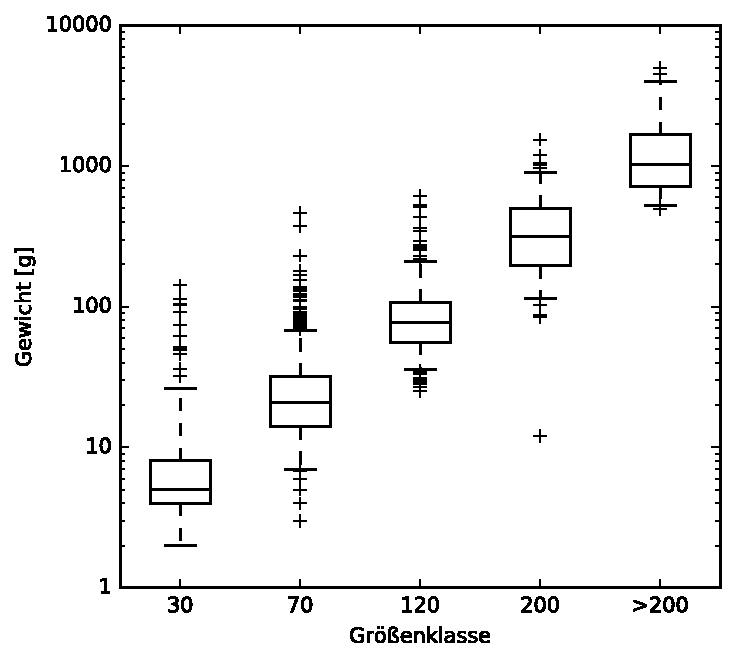
\includegraphics[height=.9\textwidth]{fig/2-2_Keramik_Gr-Gew_BoxPlt_2.pdf}
\caption{Verhältnis von Scherbengröße und Gewicht (Größenklassen siehe Anm.~\ref{ftn:Keramik_Fragmentierung}; 4218~GE).}
\label{fig:Keramik_FragmGrGew_B}
\end{subfigure}
\caption{Funde: Fragmentierung.}
\label{fig:Keramik_Typen-Fragm}
\end{figure*}

Der Anteil an unverzierten Stücken im Vergleich zu jenen GE aus dem untersuchten Materialkomplex, die Verzierungen aufweisen, variiert zwischen den Komplexen aus Oberflächensurveys und jenen aus Grabungen nur leicht. Während unverzierte Stücke in Oberflächenabsammlungen etwa 25\,\% ausmachen, sind es bei den ausgegrabenen Komplexen (Kat.-Nr.~1--19) knapp 29\,\%. Im Anschluss an die Ausgrabung der beiden Komplexe PIK~87/1 (Kat.-Nr.~8) sowie PIK~87/2 (Kat.-Nr.~9) in Pikunda am \mbox{Sangha} (Fpl.~255) wurde nachweislich unverziertes Scherbenmaterial verworfen. Im vorliegenden und ausgewerteten Fundmaterial dieser beiden Grabungen machen unverzierte Stücke immer noch 26\,\% aller GE aus. Daraus kann gefolgert werden, dass die Selektion der Stücke im Gelände die Repräsentanz des Fundinventares nur teilweise beeinträchtigt hat. Die Grabungen in Maluba am Lua (Fpl.~230; Kat.-Nr.~1--5), für die ein Aussondern \textit{nicht-diagnostischer} Stücke nicht überliefert ist, umfassten hingegen lediglich 18\,\% unverzierte Scherben. Diese Angaben legen nahe, dass die Oberflächenabsammlungen, zumindest mit Blick auf das Verhältnis von verzierten zu unverzierten Stücken, nicht grundsätzlich unrepräsentativ sind.


\subsubsection{Erhaltung}

Von den insgesamt 4217 aufgenommenen Gefäßeinheiten bestehen nur 654 aus mehr als einer Scherbe. Im Mittel bestehen die Gefäßeinheiten aus etwa 1,5 Scherben, was eine sehr starke Fragmentierung anzeigt und als Indikator für eine schlechte Erhaltung gewertet werden kann \parencite[siehe][86]{Jesse.2003}. Das mittlere Gewicht einer Gefäßeinheit liegt bei knapp 67\,g, das mittlere Gewicht der Einzelscherben bei rund 51\,g.\footnote{Der Unterschied ist wohl einzig auf die stark schiefen Verteilungen zurückzuführen.} Die Fragmentierurng der GE beziehungsweise der Zerscherbtheitsgrad der Keramik wurde unter Nutzung einer Größenklassen-Systematik aufgenommen, welche zuletzt auch bei \textcite[89]{Clist.20042005} zur Anwendung kam.\footnote{Die im Rahmen der Aufnahme genutzten Größenklassen beschreiben die Fragmentierung der Stücke mittels fünf fester Klassen (siehe \textsc{Clist}~2004/2005:~89): \textit{stark fragmentierte} beziehungsweise \textit{kleine Stücken} sind jeweils kleiner als 30\,$\times$\,30\,mm. Im ursprünglich auf \textcite[379]{Joukowsky.1980} zurückgehenden Schema liegt die kleinste Klassengrenze bei 25\,$\times$\,25\,mm \parencites[nach][]{Claes.1985}{deMaret.1985}[89]{Clist.20042005}. \textit{Mittelgroße} beziehungsweise \textit{mittelstark fragmentierte Stücke} sind zwischen  30\,$\times$\,30\,mm und 70\,$\times$\,70\,mm groß. Die nächste Klassengrenze liegt bei 120\,$\times$\,120\,mm und beschreibt \textit{gering fragmentierte} beziehungsweise \textit{große Stücke}. Stücke mit einer Größe zwischen 120\,$\times$\,120\,mm und 200\,$\times$\,200\,mm sind \textit{kaum fragmentiert} beziehungsweise \textit{groß}, während Objekte größer als 200\,$\times$\,200\,mm in der Regel große Gefäßfragmente oder ganze Gefäße widerspiegeln. Eine Dokumentation der erhalten Anteile von Gefäßprofilen und Randdurchmessern erfolgte nicht \parencite[siehe hierzu][155\,f.]{Claen.2011}. Die genannten Größenklassen wurden auch auf das nichtkeramische Fundgut, etwa Schlacken angewandt.\label{ftn:Keramik_Fragmentierung}} Während etwa 25\,\% der Keramik sehr stark fragmentiert sind -- kleiner als 30\,$\times$\,30\,mm -- sind knapp über die Hälfte der Scherben zwischen 30\,$\times$\,30\,mm und 70\,$\times$\,70\,mm groß (Abb.~\ref{KeramikFragmentierung}). Stücke größer als 70\,$\times$\,70\,mm sind seltener vertreten und machen zusammen nur etwa 20\,\% des Materials aus.


\begin{table*}[tb]
	\noindent\begin{minipage}[b]{\columnwidth}
		\centering
		{\footnotesize
			\begin{sftabular}{@{}llr@{}}
				\toprule
				\textbf{Schlüssel} & \textbf{Größenklasse} & \textbf{Durchmesser} \\
				\midrule
				VF & Very Fine & 62--125~$\mu$m \\
				F & Fine & 125--250~$\mu$m \\
				M & Medium & 250--500~$\mu$m \\
				C & Coarse & 500--1000~$\mu$m \\
				VC & Very Coarse & 1000--2000~$\mu$m \\
				\bottomrule
		\end{sftabular}}\vspace{1em}
		\captionof{table}{Keramik: Korngrößen nach der \textit{Wentworth-Grainsize-Scale}.\label{tab:Keramik_PartikelGr}}
	\end{minipage}\hfill
	\noindent\begin{minipage}[b]{\columnwidth}
		\centering
		{\footnotesize
			\begin{sftabular}{@{}lll@{}}
				\toprule
				\textbf{Schlüssel} & \textbf{Farbe} & \textbf{MUNSELL-Wert} \\
				\midrule
				S & schwarz/black & 10 YR 2/1 \\
				G & grau/grey & 10 YR 6/1 \\
				W & weiß/white & 10 YR 8/1 \\
				Bg & beige-ocker/yellow & 10 YR 8/6 \\
				Br & braun/dark reddish brown & 2.5 YR 3/4 \\
				R & rot/red & 2.5 YR 4/8--5/8 \\
				\bottomrule
		\end{sftabular}}
		\captionof{table}{Keramik: Farben der Scherbenoberflächen und -brüche.\label{tab:Keramik_Farbe}}
	\end{minipage}
\end{table*}

Die fünf Größenklassen bilden die Fragmentierung in einem zufriedenstellenden Maß ab, wie eine Gegenüberstellung mit den individuellen Scherbengewichten ergab (Abb.~\ref{fig:Keramik_FragmGrGew_B}). Trotz Ausreißern zeigen die Verteilungen, dass für jede der Größenklassen ein Gewichtsbereich angegeben werden kann, welcher sich von jenem einer anderen Größenklasse im Interquartilabstand unterscheidet. Überlappungen der Verteilungen stellen sich erst bei Betrachtung der zweifachen Standardabweichung ein.\footnote{Zur Interpretation von Box-Whisker-Plots siehe auch \textcite[81]{Hedderich.2016}. Im Fall von Abb.~\ref{fig:Keramik_FragmGrGew_B} markieren die Whiskers beziehungsweise Antennen die 2-Sigma-Standardabweichung der jeweiligen Verteilungen, während die Box das untere (25\,\%) sowie das obere Quartil (75\,\%) anzeigt und die zentrale Linie den Median markiert. Wird die einfache Standardabweichung zugrunde gelegt, lässt sich keine Überschneidung der Verteilungen beobachten.} Die Verteilungen zeigen insgesamt eine breite Streuung mit einigen Ausreißern, überlagern sich aber nur im Randbereich.


\subsubsection{Technologie}\label{sec:AufnahmeTechnologie}

Zusätzlich zu einer formalen Analyse, die sich auf morphologische Charakteristika wie Verzierung der Keramik stützt (siehe Kap.~\ref{sec:Keramiksequenz}), bildet eine tiefgreifende Auseinandersetzung mit technischen Parametern eines der Kernziele der Untersuchung. Hierfür grundlegend war die Einbeziehung von keramik-technischen Parametern in das Aufnahmesystem. Die untersuchten Kriterien gründen vornehmlich auf den Untersuchungen von \textcite{Nordstrom.1972} zu sudanesischer Keramik, welche wiederum Ausgangspunkt der neuen Studie von \textcite{Riemer.2011} zu Material aus der Dakhla-Oase in Ägypten waren, an der sich die hier vorgelegte Untersuchung orientiert. Für die Analyse der technologischen Eigenschaften der Gefäßkeramik wurde ein Katalog aus Aufnahmekriterien formuliert, welcher die folgenden Kenngrößen umfasst:
\begin{itemize*}
	\item nichtplastische Partikel
	\begin{itemize*}
		\item Größe (nach \textit{Wentworth-Grainsize-Scale})
		\item Dichte \parencites[32]{Kinne.2009}[nach][]{Hodgson.1976}
		\item Art
	\end{itemize*}
	\item Farbe des Scherben
	\begin{itemize*}
		\item Kernfarbe
		\item (Brennfarbe)
		\item Unterteilung des Scherbens in Oxidationszonen
		\item Ausbildung der Grenze zwischen Oxidationszonen
	\end{itemize*}
	\item Strukturierung der Oberfläche
\end{itemize*}

\begin{figure*}[!tb]
	\centering
	\resizebox{\textwidth}{!}{%
		{\footnotesize
\begin{sftabular}{@{}m{.02\textwidth} m{.02\textwidth} *7{>{\centering\arraybackslash}m{.1\textwidth}} m{.25\textwidth} @{}m{0pt}@{}@{}} 
 &  & \multicolumn{7}{c}{\textit{Variante}} &  &  \\
 &  & \textbf{1} & \textbf{2} & \textbf{3} & \textbf{4} & \textbf{5} & \textbf{6} & \textbf{7} & & \\
\multirow{10}{*}{\rotatebox[origin=c]{90}{\textit{Grundform} \hspace{9cm}}} & \textbf{A} & \includegraphics[height=.1\textwidth]{fig/Abb_GefFormen/G11c_Bolongo101.png} & \includegraphics[height=.1\textwidth]{fig/Abb_GefFormen/G11b_MUN87-1-0-2-6-2.png} & \includegraphics[height=.1\textwidth]{fig/Abb_GefFormen/G11a_MSG87-102-9a.png} &  &  &  &  & Flaschenförmige Gefäße & \\[.11\textwidth]
 & \textbf{B} & \includegraphics[height=.1\textwidth]{fig/Abb_GefFormen/G5_MUN87-2-1-3-8.png} & \includegraphics[height=.1\textwidth]{fig/Abb_GefFormen/G6c_msn87-101-145.png} & \includegraphics[height=.1\textwidth]{fig/Abb_GefFormen/G6b_ITN87-103-3a.png} & \includegraphics[height=.1\textwidth]{fig/Abb_GefFormen/G6a_MUN87-1-0-2-1.png} & \includegraphics[height=.1\textwidth]{fig/Abb_GefFormen/G13_MKL85-101-114.png} & \includegraphics[height=.1\textwidth]{fig/Abb_GefFormen/G4_PIK87-101-51.png} & \includegraphics[height=.09\textwidth]{fig/Abb_GefFormen/G4b.png} & hohe Gefäße & \\[.11\textwidth]
 & \textbf{C} & \includegraphics[height=.08\textwidth]{fig/Abb_GefFormen/G7a_NGB85-101-131.png} & \includegraphics[width=.1\textwidth]{fig/Abb_GefFormen/G7b_DON85-102-a.png} &  &  &  &  &  & Gefäße mit leicht konvexer Wandung und ausgeprägtem Halsbereich & \\[.11\textwidth]
 & \textbf{D} & \includegraphics[width=.1\textwidth]{fig/Abb_GefFormen/G7c_PIK87-1-2-3_1-3-7.png} & \includegraphics[width=.1\textwidth]{fig/Abb_GefFormen/G10a_NGO87-102-28-29.png} &  &  &  &  &  & Gefäße mit stark konvexer Wandung ohne ausgeprägten Halsbereich & \\[.11\textwidth]
 & \textbf{E} & \includegraphics[width=.1\textwidth]{fig/Abb_GefFormen/G3_BLK87-1-1-1-2_HS.png} & \includegraphics[width=.1\textwidth]{fig/Abb_GefFormen/G3c_MBN85-501-2.png} & \includegraphics[width=.1\textwidth]{fig/Abb_GefFormen/G1b_MUN87-2-1-3.png} & \includegraphics[width=.1\textwidth]{fig/Abb_GefFormen/G8b1_BLN85-201-b.png} & \includegraphics[width=.1\textwidth]{fig/Abb_GefFormen/G9b_DON85-102-b.png} & \includegraphics[width=.1\textwidth]{fig/Abb_GefFormen/G2d_SSL87-101-142.png} & \includegraphics[width=.1\textwidth]{fig/Abb_GefFormen/G3b_GE5_BLK87-1-1-3-1-3.png} & Gefäße mit geschweifter Wandung & \\[.11\textwidth]
 & \textbf{F} & \includegraphics[width=.1\textwidth]{fig/Abb_GefFormen/G1c_LKW87-401-1.png} & \includegraphics[width=.1\textwidth]{fig/Abb_GefFormen/G1d_MBJ_Roulettekeramik_E87-010-25.png} & \includegraphics[width=.1\textwidth]{fig/Abb_GefFormen/G1a_PIK87-101-58.png} & \includegraphics[width=.1\textwidth]{fig/Abb_GefFormen/G1a2_NGO87-102-27.png} & \includegraphics[width=.1\textwidth]{fig/Abb_GefFormen/G2e_INS87-102-2.png} & \includegraphics[width=.1\textwidth]{fig/Abb_GefFormen/G2a_NGO87-102-21.png} & \includegraphics[width=.1\textwidth]{fig/Abb_GefFormen/G2h_MND85-101-33etc.png} & Gefäße mit abknickender Wandung & \\[.11\textwidth]
 & \textbf{G} & \includegraphics[width=.1\textwidth]{fig/Abb_GefFormen/G2b_ITN87-103-9.png} & \includegraphics[width=.1\textwidth]{fig/Abb_GefFormen/G2c_MSG87-102-11.png} & \includegraphics[width=.1\textwidth]{fig/Abb_GefFormen/G2f_MSG87-101-49.png} & \includegraphics[width=.1\textwidth]{fig/Abb_GefFormen/G2g_GE2_BLK87-1-1-3-1-2.png} & \includegraphics[width=.1\textwidth]{fig/Abb_GefFormen/G2g_MUN87-1-0-2-3-1.png} & \includegraphics[width=.1\textwidth]{fig/Abb_GefFormen/G8c_Coart1907_TafXII175_neu.png} &  & Schalenförmige Gefäße mit abknickender Wandung & \\[.11\textwidth]
 & \textbf{H} & \includegraphics[width=.1\textwidth]{fig/Abb_GefFormen/G8e_kpt85-101-10.png} & \includegraphics[width=.1\textwidth]{fig/Abb_GefFormen/G8d_MBN85-501-1.png} &  &  &  &  &  & Schalenförmige Gefäße mit konvexer Wandung und einbiegendem Rand & \\[.11\textwidth]
 & \textbf{I} & \includegraphics[width=.1\textwidth]{fig/Abb_GefFormen/G8b_BYN87-101-9.png} & \includegraphics[width=.1\textwidth]{fig/Abb_GefFormen/G9a_DON85-102-120.png} & \includegraphics[width=.1\textwidth]{fig/Abb_GefFormen/G8a_BTW87-101-43.png} & \includegraphics[width=.05\textwidth]{fig/Abb_GefFormen/G8a2_ngk01_PDM87-101-105.png} &  &  &  & Schalenförmige Gefäße mit konvexer Wandung & \\[.11\textwidth]
 & \textbf{J} & \includegraphics[width=.1\textwidth]{fig/Abb_GefFormen/G12a_NGO87-102-30.png} &  &  &  &  &  &  & Tellerförmige Gefäße & \\[.11\textwidth]
%\bottomrule
\end{sftabular}
}}
	\caption{Keramik: Gefäßtypen (G6 nach \cite[Taf.~XII.175]{Coart.1907}).}
	\label{tab:Keramik_GefFormen}
\end{figure*}

\noindent Von zentraler Bedeutung sind die Eigenschaften der im Scherben enthaltenen nichtplastischen Partikel. Diese wurden entsprechend ihrer Größe und Art sowie dem Anteil, in dem sie vorkommen, aufgenommen. Die Größe der Partikel wurden entsprechend der international anerkannten \textit{Wentworth-Grainsize-Scale} \parencite[381 Tab.~1, 388 Abb.~3]{Wentworth.1922} aufgenommen, wobei fünf Größenklassen unterschieden wurden (Tab.~\ref{tab:Keramik_PartikelGr}).\footnote{Die Bestimmung der Größenklassen erfolgte makroskopisch sowie unter Zuhilfenahme einer 10-fach vergrößernden Lupe in Referenz zu einer Korngrößen-Karte der Firma \textit{Precision Core} (Denver).} Die Verrundung und Sortierung der Partikel wurden nicht systematisch aufgenommen. Der Anteil an nichtplastischen Partikeln im Scherben wurde auf Basis einer Vergleichstafel zum Abschätzen von Anteilsklassen ermittelt \parencites[32]{Kinne.2009}[nach][]{Hodgson.1976}. Die Ansprache der Art der Partikel erfolgte basierend auf makroskopisch sichtbaren Kriterien und den Erfahrungen des Autors.

Zusätzlich zu diesen Eigenschaften der im Scherben beobachtbaren nichtplastischen Partikel erfolgte eine systematische Aufnahme der farblichen Zonierung der Stücke. Die farblichen Abstufungen der Keramik wurden mittels einer fünf Zonen umfassenden Unterteilung der Stücke sowie sechs Farbklassen\footnote{Zur Frage der Nutzung von Farbklassen entgegen der Aufnahme individueller MUNSELL-Farbwerte sei an dieser Stelle exemplarisch auf die Diskussion durch \textcite[38]{Keding.1997} verwiesen.} umfassenden Systematik erfasst (Tab.~\ref{tab:Keramik_Farbe}). Die fünf unterschiedenen Zonen gliedern sich in die äußere und innere Oberfläche des Stücks sowie drei Zonen im Profil beziehungsweise Bruch: den Bereich nahe der Außen- sowie Innenseite sowie der Kernbereich selbst. Die Oberflächenfarbe wurde als \textit{basic surface colour} nach \textcite[44\,f.]{Nordstrom.1972} aufgenommen. Die Ausbildung der Grenze zwischen den farblichen Zonen im Profil wurde in Anlehnung an \textcite[27]{Kinne.2009} umschreibend erfasst.

\begin{figure*}[p]
	\noindent\begin{minipage}[b]{\columnwidth}
		\centering
		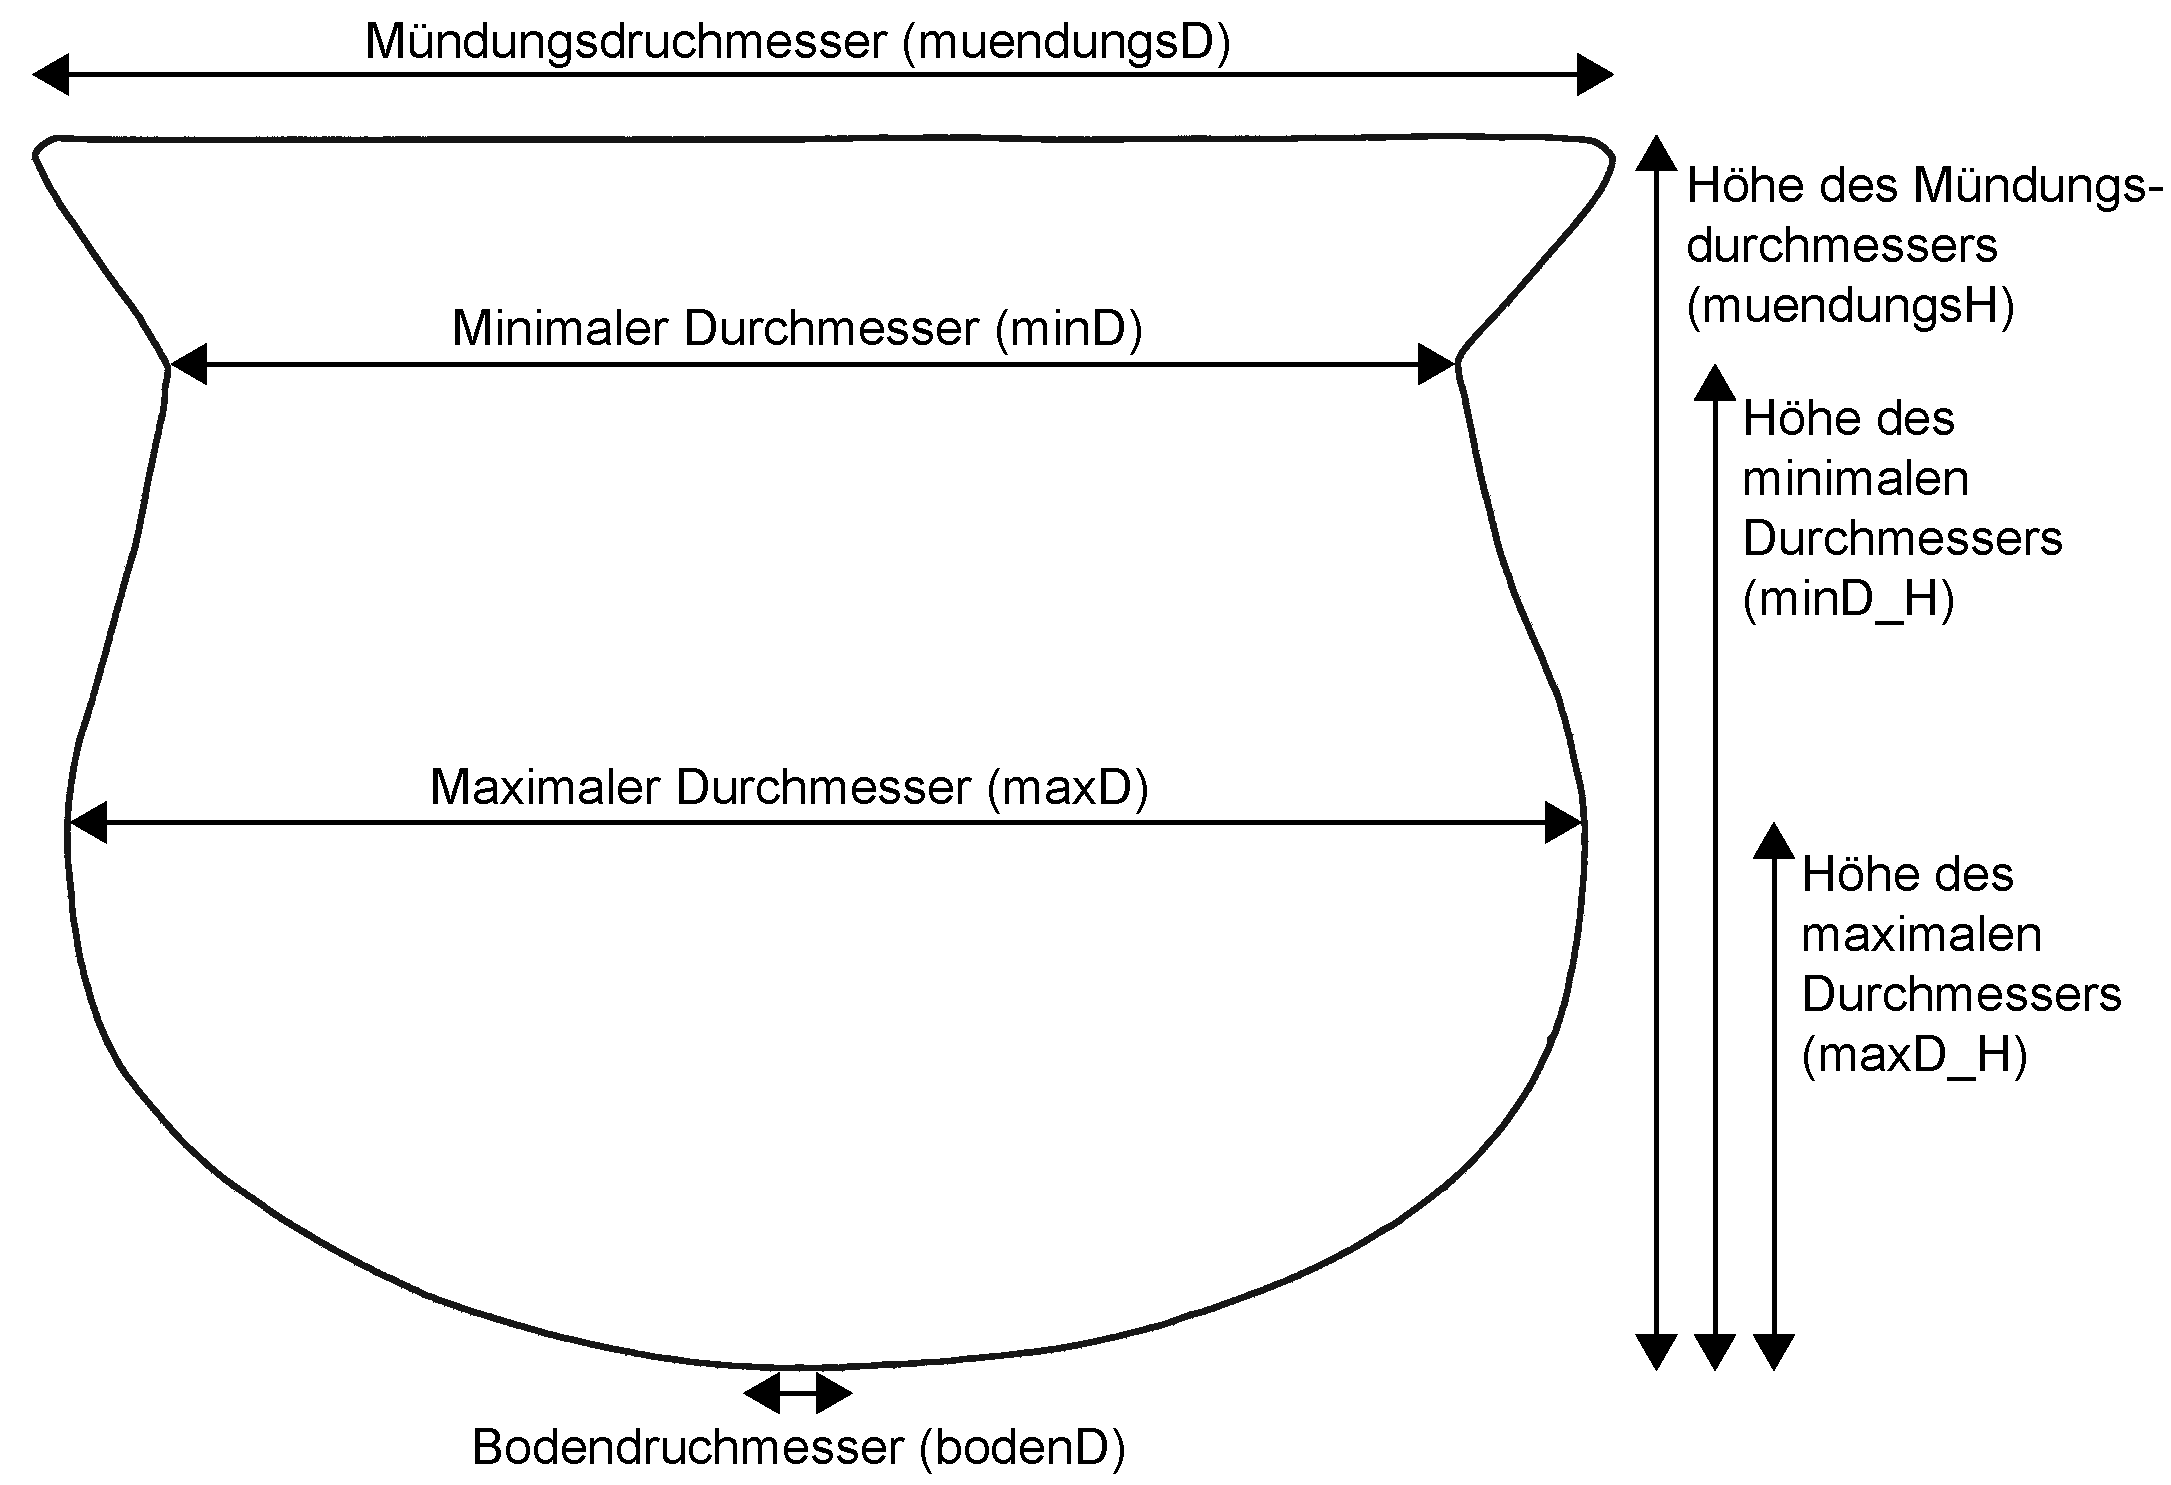
\includegraphics[width=\textwidth]{fig/GefaesseAbmessungenSystematik.pdf}
		\captionof{figure}{Keramik: Aufnahmeschema für die Gefäßabmessungen \parencite[nach][]{Wicke.2011}.\label{fig:GefAbmessungen_Schema}\\}
		\vspace{4cm}\captionof{figure}{Keramik: Systematik der Gefäßzonen, die für die Beschreibung morphologischer Ausprägungen sowie Verzierungen herangezogen wurde.\label{fig:Keramik_VerzZonen}}
	\end{minipage}\hfill
	\noindent\begin{minipage}[b]{\columnwidth}
		\centering
		\includegraphics[width=\textwidth]{fig/Keramik_Systematik_Verzierungszonen.pdf}
	\end{minipage}
\end{figure*}

Die Oberflächenstruktur der Stücke wurde unter Referenz auf eine grobe, subjektive Ansprache als \textit{glatt}, \textit{leicht rau} oder \textit{rau} erfasst. Die bei der Keramik der Mandombe-Gruppe (Kap.~\ref{sec:MDB-Gr}) beobachtete Schlicker-Rauung der Gefäßunterteile (siehe Taf.~47.24) wurde als entsprechende Eigenschaft der Oberfläche erfasst. Spezifische Behandlungen der Oberfläche, wie Engoben, wurden hingegen gesondert, gemeinsam mit Anhaftungen an den Stücken aufgenommen. Für diese Oberflächenbehandlungen wurde keine Systematik herangezogen, die Beobachtungen wurden beschreibend in der Datenbank verzeichnet.

Die sich aus diesen technischen Eigenschaften des Scherbens ergebenden Gruppen wurden als \textit{Fabrics} konzeptualisiert und werden in Kap.~\ref{sec:Herstellung2_Fabric} detailliert besprochen.

%\pagebreak
\subsubsection{Form}

\paragraph{Gefäßform}\hspace{-.5em}|\hspace{.5em}%
Im Rahmen der Auswertung der Gefäßkeramik konnten zehn verschiedene Grundformen unterschieden werden (Abb.~\ref{tab:Keramik_GefFormen} A--J). Diese ließen sich weiter in Varianten (Abb.~\ref{tab:Keramik_GefFormen} 1--7) differenzieren, wodurch sich 41 Gefäßtypen ableiten ließen. Die gewählte Systematisierung der beobachteten Formen war für die angestrebte diachrone Untersuchung unerlässlich, da sich Gefäßformen einerseits zwar im Zeit-Raum-Kontinuum verändern, andererseits sich die Grundformen aber auch immer wiederholen \parencite[86]{Saev.2015}. Die von \textcite[39\, f.]{Wotzka.1995} genutzte Systematisierung, die nur grobe Grundformen wie Topf, Schale, Teller oder Flasche kennt und zusammengenommen 115 Gefäßtypen umfasst, konnte aufgrund ihrer spezifisch auf das Material aus dem Inneren Kongobecken zugeschnittenen Ausprägung nicht übernommen werden.\columnbreak

Insgesamt war bei 2178 Gefäßeinheiten (41\,\%) eine Ansprache der Gefäßform möglich. Die Proportionen der GE wurden, wo das Abnehmen der entsprechenden Maße möglich war, unter Einsatz von sieben Messstrecken systematisch erfasst \parencite[Abb.~\ref{fig:GefAbmessungen_Schema}; siehe][]{Wicke.2011}.\footnote{Im Laufe der Materialaufnahme erwies es sich als problematisch, dass das verwendete Aufnahmeschema für die Höhenwerte von der Standfläche eines Gefäßes ausgeht. Bei einer hohen Zahl von GE fehlte der untere Gefäßteil. Die Höhen der Randabschlüsse und minimaler sowie maximaler Durchmesser ließen sich so nicht aufnehmen. Da das Problem erst spät in der Aufnahme zu Tage trat, wurde von einer systematischen Anpassung der Vermessung abgesehen. In Fällen, in denen eine Bestimmung der fehlenden Partie in akzeptabler Weise möglich schien, wurde die hypothetische Position der Standfläche rekonstruiert und protokolliert.} Die Abmessungen wurden mit einer Messgenauigkeit von 0,5\,cm aufgenommen, wodurch die Proportionen der von Hand aufgebauten Keramik des Arbeitsgebiets angemessen repräsentiert sind.\footnote{Der Unterschied zwischen Mündungsweite, der tatsächlichen Gefäßöffnung und dem Randdurchmesser wurde nicht ausdifferenziert \parencite[siehe][88]{Saev.2015}.}

Die morphologischen Ausprägungen einzelner GE, wie auch die Verzierung (siehe Kap.~\ref{sec:AufnahmeVerzierungen}), wurden mit Bezug auf vordefinierte Gefäßzonen aufgenommen (Abb.~\ref{fig:Keramik_VerzZonen}). Die Abgrenzung der einzelnen Zonen wurde auf Basis markanter Wendepunkte am Profilverlauf der GE vorgenommen.

\begin{figure*}[p]
	\noindent\begin{minipage}[b]{\columnwidth}
		\centering
		{\footnotesize
			\begin{sftabular}{@{} >{\centering\arraybackslash} m{.01\textwidth} >{\centering\arraybackslash} m{.19\textwidth} >{\centering\arraybackslash} m{.19\textwidth} >{\centering\arraybackslash} m{.19\textwidth} >{\centering\arraybackslash} m{.19\textwidth}@{}}
				%\toprule
				& \textbf{1} & \textbf{2} & \textbf{3} & \textbf{4} \\
				%\midrule
				\textbf{A} & 
\includegraphics[height=.2\textwidth]{fig/Abb_RandFormen/A1.pdf} & 
\includegraphics[height=.2\textwidth]{fig/Abb_RandFormen/A2.pdf} & 
\includegraphics[height=.2\textwidth]{fig/Abb_RandFormen/A3.pdf} & 
\includegraphics[height=.2\textwidth]{fig/Abb_RandFormen/A4.pdf} \\
				\textbf{B} & \includegraphics[height=.2\textwidth]{fig/Abb_RandFormen/B1.pdf} & \includegraphics[height=.2\textwidth]{fig/Abb_RandFormen/B2.pdf} & \includegraphics[height=.2\textwidth]{fig/Abb_RandFormen/B3.pdf} & \\
				\textbf{C} & \includegraphics[height=.2\textwidth]{fig/Abb_RandFormen/C1.pdf} & \includegraphics[height=.2\textwidth]{fig/Abb_RandFormen/C2.pdf} & \includegraphics[height=.2\textwidth]{fig/Abb_RandFormen/C3.pdf} & \\
				%\bottomrule
		\end{sftabular}}\vspace{2em}
		\captionof{figure}{Keramik: Unterschiedene Randformen. Grundformen A--B als Zeilen und Varianten in Spalten.\label{tab:Keramik_RandFormen}}
	\end{minipage}\hfill
	\noindent\begin{minipage}[b]{\columnwidth}
		\centering
		{\footnotesize
			\begin{sftabular}{@{}m{.1\textwidth}m{.1\textwidth}m{.69\textwidth}@{}}
				\toprule
				& \textbf{Typ} & \textbf{Beschreibung} \\
				\midrule
				\includegraphics[height=.1\textwidth]{tbl/Tab_MdgFormen/M1_ATANGANA1988OkoloS162_1.png} & M1 & rund \\
				\includegraphics[height=.1\textwidth]{tbl/Tab_MdgFormen/M2_ATANGANA1988OkoloS162_2.png} & M2 & spitz \\
				\includegraphics[height=.1\textwidth]{tbl/Tab_MdgFormen/M3_ATANGANA1988OkoloS162_3.png} & M3 & gerade/flach/horizontal abgestrichen \\
				\includegraphics[height=.1\textwidth]{tbl/Tab_MdgFormen/M4_ATANGANA1988OkoloS162_4.png} & M4 & gerillt \\
				\includegraphics[height=.1\textwidth]{tbl/Tab_MdgFormen/M5_schraegAussen.png} & M5 & schräg nach außen abgestrichen \\
				\includegraphics[height=.1\textwidth]{tbl/Tab_MdgFormen/M6_schraegInnen.png} & M6 & schräg nach innen abgestrichen \\
				\bottomrule
		\end{sftabular} }
		\captionof{table}{Keramik: Übersicht der Randlippe \parencite[erweitert nach][162\,f. Tab.~24]{Atangana.1988}.\label{tab:MdgFormen}}
	\end{minipage}
\end{figure*}

\begin{figure*}[!tb]
	\centering
	\includegraphics[width=.95\textwidth]{fig/Wotzka1995_440Taf6_modDS.jpg}
	\caption{Keramik: Bodenformen \parencite[nach][440 Taf.~6]{Wotzka.1995}.}
	\label{fig:Keramik_BodenFormen}
\end{figure*}

\paragraph{Randform}\hspace{-.5em}|\hspace{.5em}\label{sec:Randform}
Die Aufnahme der Ränder erfolgte gemäß einer Systematik, die sich in erster Linie an der grundsätzlichen Ausrichtung des Randes orientiert. Differenziert wurden parallele, ausbiegende sowie einbiegende Ränder (Abb.~\ref{tab:Keramik_RandFormen}: A--C). Innerhalb dieser Grundtypen wurden mehrere charakteristische Varianten unterschieden. Parallele Ränder können neben der einfachen Grundform auch als umgelenkte, T-förmige sowie verdickte Formen vorkommen (Abb.~\ref{tab:Keramik_RandFormen}: A2--A4). Aus- wie einbiegende Ränder wurden noch in konkave sowie konvexe Varianten unterschieden (Abb.~\ref{tab:Keramik_RandFormen}: B2--B3, C2--C3):

\vspace{1em}
\noindent\begin{tabular}{@{}ll@{}}
A1 & parallel \\
A2 & umgelegt \\
A3 & T-förmig \\
A4 & verdickt \\
B1 & ausbiegend \\
B2 & konkav ausbiegend \\
B3 & konvex ausbiegend \\
C1 & einbiegend \\
C2 & konkav einbiegend \\
C3 & konvex einbiegend \\
\end{tabular}
\vspace{1em}

\noindent An die Grundform angefügte Parameter \enquote{.1} sowie \enquote{.2} zeigen \textit{kurze} beziehungsweise \textit{lange} Varianten der entsprechenden Randform an. Spezifischere und diagnostische Variationen der Grundformen wurden im weiteren Verlauf der Aufnahme durch Hinzusetzen individueller Zählnummern, beginnend ab dem Schlüssel-Zusatz \enquote{.3}, angefügt. Insgesamt ergaben sich zehn Grundformen der Randgestaltung (Abb.~\ref{tab:Keramik_RandFormen}) sowie 26 unterscheidbare Variationen.\footnote{Wie bereits bei den Gefäßformen (Abb.~\ref{tab:Keramik_GefFormen}) spiegelt die gewählte Form der Systematisierung das Bestreben wider, die Aufnahme des Untersuchungsmaterials vor dem Hintergrund der dieser Arbeit zugrundeliegenden diachronen Fragestellungen durchzuführen.}

Die häufigste Randform, die einfach ausbiegenden Ränder (B1), macht 24,8\,\% aller bestimmten Randformen aus, gefolgt von konkav ausbiegenden Rändern (B2), die in 13,3\,\% aller Fälle beobachtet wurden. Die kurze Variante gerade ausbiegender Ränder (B1.1) macht 11,7\,\% aus, während parallel, gerade aufsteigende Ränder (A1) auf einen Anteil von 10\,\% kommen. Alle übrigen Varianten liegen jeweils im Bereich von unter 7\,\%. Zusammengenommen repräsentieren diese, einzeln nur selten vertretenen Formen, 40\,\% der aufgenommen Gefäßränder. Werden die unterschiedenen Variationen den jeweiligen Grundformen (Abb.~\ref{tab:Keramik_RandFormen}) zugerechnet, sind insgesamt 68,5\,\% aller Rändern ausbiegend (B), während 25\,\% parallel (A) verlaufen und nur 6,5\,\% einbiegend (C) sind.

\paragraph{Randlippe}\hspace{-.5em}|\hspace{.5em}%
Die Ausprägung der Randlippe, in diesem Zusammenhang auch \textit{Gefäßmündung} genannt, wurde in Anlehnung an die von \textcite[162f Tab.~24]{Atangana.1988} genutzte Systematik losgelöst von der Randform aufgenommen (Tab.~\ref{tab:MdgFormen}).\footnote{\textcite[48]{Wotzka.1995} erfasste die Ausprägung der Randlippe nicht separat, sie bildete vielmehr eine mögliche Variation des \textit{Randtyps} ab. Ähnlich ging auch \textcite[110]{Jesse.2003} vor.} Die Einteilung Atanganas wurde dabei um die beiden Formen M5 sowie M6, die schräg nach außen oder innen abgestrichene Randlippen widerspiegeln, erweitert. Die Varianten M1 bis M5 sind jeweils in Häufigkeiten zwischen 13,5 bis 26,4\,\% vertreten, schräg nach innen abgestrichene Randlippen des Typs M6 kommen mit nur 3,9\,\% deutlich seltener vor.

\paragraph{Bodenform}\hspace{-.5em}|\hspace{.5em}\label{sec:Bodenform}
Die Unterscheidung der Ausformung des Bodens gründete sich auf die von \textcite[440 Taf.~6]{Wotzka.1995} aufgestellten Systematik, die um eine Form B15 erweitert wurde. Die neue Bodenform B15 beschreibt Gefäße, die auf einzelnen \textit{Füßchen} stehen. Im untersuchten Material fanden sich lediglich zwei GE mit drei symmetrisch am Unterteil eines ansonsten rund ausgeformten Bodens angebrachten \textit{Füßchen} (Taf.~1.2, 2.1). Im Detail wurden folgende Bodenformen unterschieden (Abb.~\ref{fig:Keramik_BodenFormen}):
\setlength\LTleft{0pt}
\vspace{.25em}
\noindent\begin{tabular}{@{}ll@{}}
	B1 & Rundboden \\
	B2 & Linsenboden \\
	B3 & Spitzboden \\
	B4 & einfacher Flachboden \\
	B5 & innen aufgewölbter Flachboden  \\
	B6 & Flachboden mit konkaver Standfläche \\
	B7 & Omphalosboden \\
	B8 & Riefenprofilierter Flachboden \\
	B9 & Profiliert abgesetzter Flachboden \\
	B10 & Riefenabgesetzter Flachboden \\
	B11 & abgesetzter Flachboden \\
	B12 & Flachboden mit einziehender Unterseite\\
\end{tabular}
%\vspace{1em}

%\setlength\LTleft{0pt}
\vspace{.25em}
\noindent\begin{tabular}{@{}ll@{}}
	B13 & Standring / Hohlfuß \\
	B14 & massiver Standfussboden \\
	B15 & Boden mit abgesetzten Standfüßen \\
\end{tabular}
\vspace{1em}

\noindent Insgesamt konnte die Bodenform lediglich bei 6\,\% aller GE angesprochen werden. Dieser geringe Anteil liegt zu einen gewissen Grad an den Schwierigkeiten, die mit der Ansprache runder Böden (B1) verbunden sind, die leicht als Fragmente der Gefäßwandung fehlinterpretiert werden können. Zusammengenommen machen runde Böden (B1) knapp 49\,\% aller bestimmter Böden aus. Einfache Flachböden (B4) kommen mit 24\,\% am zweithäufigsten vor. Gefolgt werden sie von Linsenböden (B2) mit 6\,\%, Standringböden mit Hohlfuß (B13) mit ebenfalls 6\,\% sowie 5\,\% Flachböden mit konkaver Standfläche (B6). Die übrigen Formen kommen lediglich als Einzelfunde beziehungsweise bei weniger als zehn GE vor. Der von \textsc{Wotzka} (ebd. 440 Taf.~6) beschriebe Typ B14 wurde nicht beobachtet.

\subsubsection{Verzierung}\label{sec:AufnahmeVerzierungen}

Die Verzierungen der Keramik wurden für jede Gefäßeinheit individuell und in Referenz zur Gefäßregion aufgenommen (siehe Abb.~\ref{fig:Keramik_VerzZonen}).\footnote{Während formale Ansprachen wie die Gefäßform in einer 1:n-Beziehung in einer Datenbank abgebildet werden können (eine GE kann lediglich eine Gefäßform oder Randform aufweisen), können verschiedene Verzierungen auf verschiedenen Gefäßbereichen unterschiedlich häufig vorkommen. Die vorliegende Kardinalität der Entitätstypen \textit{Objekt}, \textit{Gefäßposition} und \textit{Verzierungselement} können in dem genutzten relativen Datenbankschema nicht direkt abgebildet werden. Die Entitäten jeder dieser Entitätstypen können mit beliebig vielen Entitäten der anderen beiden Entitätstypen in Beziehung stehen. Konkret ist hiermit gemeint, dass eine GE an verschiedenen Stellen auch mehrere Verzierungselemente aufweisen kann. Als Lösung wird eine Konkordanztabelle genutzt, welche die Primärschlüssel der genannten Entitätstypen als Fremdschlüssel-Paare beinhaltet. Die Beziehungen der drei Entitätstypen werden im Datenmodell durch drei getrennte 1:n-Beziehungen aufgelöst.} Basierend auf der Kombination aus Verzierungstechnik und -motiv wurden Verzierungselemente erarbeitet (Tab.~\ref{tab:Verzierungselemente}; Abb.~\ref{fig:Keramik_VerzSystematik}).\footnote{Die Klassifizierung der einzelnen Verzierungselemente lehnt sich dabei stark an \textsc{Wotzka} (1995) an, nimmt aber auch Aspekte aus Systematiken für die Bandkeramik \parencites{Stehli.1973}{Stehli.1977}{Kneipp.1998} und das südfranzösische Frühneolithikum auf \parencites[126\,f. Abb.~3]{Manen.2002}[auch bei][]{Linstadter.2013}. Die grafische Zusammenstellung der Klassifizierung in Abb.~\ref{fig:Keramik_VerzSystematik} folgt der Darstellungsweise von \textcite[80\,f. Abb.~39]{Keding.1997}.} Diese bilden in der Aufnahme der Verzierungen wie deren Auswertung die analytische Grundeinheit.

\begin{figure*}[p]
 \centering
 \includegraphics[width=.85\textwidth]{fig/VerzierungenSystematik.pdf}
 \caption{Keramik: Verzierungstechniken, Verzierungswerkzeuge und Verzierungselemente.}
 \label{fig:Keramik_VerzSystematik}
\end{figure*}

%\end{multicols}
%\afterpage{%
%\clearpage
\begin{table*}[p]

\begin{multicols}{2}
\noindent
{\scriptsize\begin{sftabular}{@{}m{.05\columnwidth} m{.1\textwidth} m{.63\columnwidth}@{}}
\toprule
\multicolumn{2}{@{}l@{}}{\textbf{Schlüssel}} &  \textbf{Kurzbeschreibung} \\
\midrule
01.1 & \includegraphics[width=.1\textwidth]{tbl/Tab_VerzElemente/V03a_PIK87-1-7-1.png} & \textit{Schachbrett}-Muster aus horizontalen und vertikalen Ritzlinien \\
01.2 & \includegraphics[width=.1\textwidth]{tbl/Tab_VerzElemente/V03b_PIK87-1-6-16.png} & \textit{Schachbrett}-Muster aus diagonalen Ritzlinien \\
01.3 & \includegraphics[width=.1\textwidth]{tbl/Tab_VerzElemente/V03c_PIK87-1-8-6.png} & \textit{Schachbrett}-Muster aus horizontalen und diagonalen Ritzlinien \\
01.4 & \includegraphics[width=.1\textwidth]{tbl/Tab_VerzElemente/V03d_PIK87-1-9-7.png} & \textit{Schachbrett}-Muster aus diagonalen und vertikalen Ritzlinien \\
01.5 & \includegraphics[width=.1\textwidth]{tbl/Tab_VerzElemente/V01b_PIK87-1-5-7.png} & Wellenlinien \\
01.6 & \includegraphics[width=.1\textwidth]{tbl/Tab_VerzElemente/V12a1_MSG87-102-8.png} & Zickzack-Linien \\
01.7 & \includegraphics[width=.1\textwidth]{tbl/Tab_VerzElemente/V12c_Gef9_CAM07-3-1-278-306.png} & Rillen in Fischgrät-Muster \\
01.8 & \includegraphics[width=.1\textwidth]{tbl/Tab_VerzElemente/V04d_PIK87-101-43-46.png} \includegraphics[width=.1\textwidth]{tbl/Tab_VerzElemente/V04e_NGO87-102-28-29.png} & Rillen gefüllte Flächen (Dreiecke, Rauten u.~a.) \\
01.9 & \includegraphics[width=.1\textwidth]{tbl/Tab_VerzElemente/V10a_PIK87-101-51.png} & feine vertikale oder horizontale Rillen \\
01.10 & \includegraphics[width=.1\textwidth]{tbl/Tab_VerzElemente/V10b_PIK87-101-40.png} & feine diagonale Rillen \\
01.11 & \includegraphics[width=.1\textwidth]{tbl/Tab_VerzElemente/V11b1_LKW87-186-1-2-5.png} & Muster aus überkreuzten Rillen \\
02.1 & \includegraphics[width=.1\textwidth]{tbl/Tab_VerzElemente/V01a_PIK87-1-8-6.png} & horizontale Riefen \parencite[siehe Muster \enquote{ISpeg5} von][251 Abb. 30.5 ]{GouemGouem.20102011} \\
02.2 & \includegraphics[width=.1\textwidth]{tbl/Tab_VerzElemente/V01c_PIK87-1-8-6.png} & vertikale Riefen \\
\bottomrule
\end{sftabular}}

\noindent
{\scriptsize\begin{sftabular}{@{}m{.05\columnwidth} m{.1\textwidth} m{.63\columnwidth}@{}}
\toprule
\multicolumn{2}{@{}l@{}}{\textbf{Schlüssel}} &  \textbf{Kurzbeschreibung} \\
\midrule
02.3 & \includegraphics[width=.1\textwidth]{tbl/Tab_VerzElemente/V01e_PIK87-1-8-6.png} & diagonale Riefen \\
02.4 & \includegraphics[width=.1\textwidth]{tbl/Tab_VerzElemente/V01e2_MLB85-1-3-2-5-35.png} & horizontales Band aus kurzen diagonalen Riefen \\
02.5 & \includegraphics[width=.1\textwidth]{tbl/Tab_VerzElemente/V01d_PIK87-101-7.png} & gebogene Riefen \\
02.6 & \includegraphics[width=.1\textwidth]{tbl/Tab_VerzElemente/V01f_MUN87-2-1-1-5-2.png} & spitz zusammenlaufende gebogene Riefen \\
02.7 & \includegraphics[width=.1\textwidth]{tbl/Tab_VerzElemente/V04c_PIK87-1-3-9.png} & sehr breite Riefen (\textgreater\,5\,mm) \\
03.1 & \includegraphics[width=.1\textwidth]{tbl/Tab_VerzElemente/V06e.png} & große Eindrücke, Fingereindrücke \\
04.1 & \includegraphics[width=.1\textwidth]{tbl/Tab_VerzElemente/V02a_PIK87-1-8-6.png} & Wiegeband mit Kamm \\
04.2 & \includegraphics[width=.1\textwidth]{tbl/Tab_VerzElemente/V02b_MUN87-2-1-1-4-2.png} & Wiegeband (siehe Muster \enquote{IIIPla1z} von \textsc{Gouem Gouem} 2010/2011: 117 Abb. 9.3.a ) \\
04.3 & \includegraphics[width=.1\textwidth]{tbl/Tab_VerzElemente/V05e_INS87-102-2.png} & gruppierte Eindrücke \\
04.4 & \includegraphics[width=.1\textwidth]{tbl/Tab_VerzElemente/V05f_SSL87-101-143.png} & gegenständige Eindrücke \\
04.5 & \includegraphics[width=.1\textwidth]{tbl/Tab_VerzElemente/V05j_SSL87-101-5.png} & kleine Flächen aus gegenständigen, halbrunden Eindrücken \\
04.6 & \includegraphics[width=.1\textwidth]{tbl/Tab_VerzElemente/V05h_DON85-102-a.png} & flache, winkelige Eindrücke \\
04.7 & \includegraphics[width=.1\textwidth]{tbl/Tab_VerzElemente/V05i1_MLB85-1-2-3.png} & kleine Kreisaugen-Eindrücke \\
& & \\[1mm]
\bottomrule
\end{sftabular}}
\end{multicols}
\caption{Keramik: Verzierungselemente. Für die ersten beiden Stellen der Schlüsselzahl -- die  Verzierungstechnik -- siehe \textsc{Wotzka} (1995: 44 Tab.~3).}
\label{tab:Verzierungselemente}
\end{table*}

\addtocounter{table}{-1}
\begin{table*}[p]
\begin{multicols}{2}
\noindent
{\scriptsize\begin{sftabular}{@{}m{.05\columnwidth} m{.1\textwidth} m{.63\columnwidth}@{}}
\toprule
\multicolumn{2}{@{}l@{}}{\textbf{Schlüssel}} &  \textbf{Kurzbeschreibung} \\
\midrule
04.8 & \includegraphics[width=.1\textwidth]{tbl/Tab_VerzElemente/V09l_MKA87-102-1.png} & dreieckige Eindrücke/Dreieckstempel \\
04.9 & \includegraphics[width=.1\textwidth]{tbl/Tab_VerzElemente/V09j_MIS87-101-56.png} & flächig angeordnete, horizontale Bänder kleiner Eindrücke \\
04.10 & \includegraphics[width=.1\textwidth]{tbl/Tab_VerzElemente/V09k_MIS87-101-56.png} & lose flächig verteilte kleine Eindrücke \\
04.11 & \includegraphics[width=.1\textwidth]{tbl/Tab_VerzElemente/V09i2_MKL85-101-114.png} & runde bis leicht ovale Eindrücke \\
04.12 & \includegraphics[width=.1\textwidth]{tbl/Tab_VerzElemente/V09a1_PIK87-1-14-1.png} & diagonale Eindrücke \\
04.13 & \includegraphics[width=.1\textwidth]{tbl/Tab_VerzElemente/V09n_SSL87-101-19.png} & leicht gewellte Bänder aus diagonalen oder vertikalen Eindrücken \\
04.14 & \includegraphics[width=.1\textwidth]{tbl/Tab_VerzElemente/V09a2_DON85-102-120.png} & horizontales oder vertikales Band aus linearen Eindrücken \\
04.15 & \includegraphics[width=.1\textwidth]{tbl/Tab_VerzElemente/V09b_PIK87-1-8-10.png} & vertikale Eindrücke \\
04.16 & \includegraphics[width=.1\textwidth]{tbl/Tab_VerzElemente/V09c1_PIK87-1-13-1.png} \includegraphics[width=.1\textwidth]{tbl/Tab_VerzElemente/V09c2_DON85-102-117.png} & Eindrücke in Rillen (siehe Muster \enquote{ISpeg5/ISpeg11} bei \textsc{Gouem Gouem} 2010/2011251, 251 Abb. 30.5) \\
04.17 & \includegraphics[width=.1\textwidth]{tbl/Tab_VerzElemente/V12b_INS87-102-2.png} & gegenständige Dreiecke in horizontalem Band \\
04.18 & \includegraphics[width=.1\textwidth]{tbl/Tab_VerzElemente/V11b2_DON85-102-126.png} & Bänder aus x-förmigen Eindrücken \\
04.19 & \includegraphics[width=.1\textwidth]{tbl/Tab_VerzElemente/V09h1_PDM87-101-12.png} & lange gebogene Eindrücke in Reihen \\
04.20 & \includegraphics[width=.1\textwidth]{tbl/Tab_VerzElemente/V09h2_MIT87-102-19.png} & kurze gebogene Eindrücke (Fingernagel) \\
04.21 & \includegraphics[width=.1\textwidth]{tbl/Tab_VerzElemente/V05i3_MBA11-1-1_DSC_0507_b.png} & Eindrücke mit Kaurischnecken oder Imitation \\
& & \\
\bottomrule
\end{sftabular}}

\noindent
{\scriptsize\begin{sftabular}{@{}m{.05\columnwidth} m{.1\textwidth} m{.63\columnwidth}@{}}
\toprule
\multicolumn{2}{@{}l@{}}{\textbf{Schlüssel}} &  \textbf{Kurzbeschreibung} \\
\midrule
05.1 & \includegraphics[width=.1\textwidth]{tbl/Tab_VerzElemente/V02c_PDM87-101-125.png} & diagonaler Kammeindruck \\
05.2 & \includegraphics[width=.1\textwidth]{tbl/Tab_VerzElemente/V12a3_MKL85-101-105.png} & Band aus zickzackartig angeordneten Kammeindrücken \\
05.3 & \includegraphics[width=.1\textwidth]{tbl/Tab_VerzElemente/V05a_PIK87-1-2-5.png} & Kammeindruck-Bänder \\
05.4 & \includegraphics[width=.1\textwidth]{tbl/Tab_VerzElemente/V05b_PIK87-101-8.png} & flächiger Kammeindruck \\
08 & \includegraphics[width=.1\textwidth]{tbl/Tab_VerzElemente/V07_MUN87-1-0-2-3-6.png} & \textit{Bnfwa-nfwa} \parencite[Muster: siehe][109--111]{Wotzka.1995} \\
09.1 & \includegraphics[width=.1\textwidth]{tbl/Tab_VerzElemente/V06a1_PIK87-1-2-5.png} & Knubben \\
09.2 & \includegraphics[width=.1\textwidth]{tbl/Tab_VerzElemente/V06b_PIK87-101-8.png} & Plastische Leiste \\
12 & \includegraphics[width=.1\textwidth]{tbl/Tab_VerzElemente/V14_Wotzka1995_Taf91-4.png} & Mattenabdruck \\
13.1 & \includegraphics[width=.1\textwidth]{tbl/Tab_VerzElemente/V13_Gef3_CAM07-12-II-2.png} & Durchlochung der Gefäßwandung \\
14.1 & \includegraphics[width=.1\textwidth]{tbl/Tab_VerzElemente/VB1_YUM87-103-2.png} & Schwarze bis dunkelgraue Bemalung. Die Bemalung erfolgt ausschließlich in Streifen. Eine flächige Bemalung größerer Abschnitte eines Gefäßes wurde nicht beobachtet. \\
14.2 & \includegraphics[width=.1\textwidth]{tbl/Tab_VerzElemente/Vb2_BBS87-Herdgef_E87-04-4.png} & Rote Bemalung. Die Bemalung erfolgt ausschließlich in Streifen sowie in Riefen. Eine flächige Bemalung größerer Abschnitte eines Gefäßes wurde nicht beobachtet. \\
15.1 & \includegraphics[width=.1\textwidth]{tbl/Tab_VerzElemente/V04a_PIK87-1-3-5.png} & diagonaler Kammstrich \\
15.2 & \includegraphics[width=.1\textwidth]{tbl/Tab_VerzElemente/V04b_PIK87-1-2-225.png} & überkreuzter Kammstrich \\
& & \\[1.5mm]
\bottomrule
\end{sftabular}}
\end{multicols}
\caption{Keramik: Verzierungselemente. Für die ersten beiden Stellen der Schlüsselzahl -- die  Verzierungstechnik -- siehe \textsc{Wotzka} (1995: 44 Tab.~3).}
%\label{tab:Verzierungselemente}
\end{table*}

\addtocounter{table}{-1}
\begin{table*}[!tb]
\begin{multicols}{2}
\noindent
{\scriptsize\begin{sftabular}{@{}m{.05\columnwidth} m{.1\textwidth} m{.63\columnwidth}@{}}
\toprule
\multicolumn{2}{@{}l@{}}{\textbf{Schlüssel}} &  \textbf{Kurzbeschreibung} \\
\midrule
15.3 & \includegraphics[width=.1\textwidth]{tbl/Tab_VerzElemente/V05i2a_PIK87-101-17.png} \includegraphics[width=.1\textwidth]{tbl/Tab_VerzElemente/V05i2b_MTB85-101-12.png} & in Kammstrich-Technik hergestellte konzentrische, teilweise sich überlagernde Kreis-Muster \\
17.1 & \includegraphics[width=.1\textwidth]{tbl/Tab_VerzElemente/V06a2_MLB85-101-18.png} & Ösen \\
17.2 & \includegraphics[width=.1\textwidth]{tbl/Tab_VerzElemente/V06a3_LIB85-101-50.png} & Henkel \\
20.1 & \includegraphics[width=.1\textwidth]{tbl/Tab_VerzElemente/V08m_NGA87-101-22.png} & unklar, möglicherweise Mattenabdruck \\
20.2 & \includegraphics[width=.1\textwidth]{tbl/Tab_VerzElemente/V08n_MBK85-101-11.png} & unklar, möglicherweise Textilabdruck \\
21.1 & \includegraphics[width=.1\textwidth]{tbl/Tab_VerzElemente/V08a_BBL85-101-61.png} & \textit{knotted strip} \parencite[Muster: siehe][191 Abb.~1,C]{LivingstoneSmith.2007} \\
21.2 & \includegraphics[width=.1\textwidth]{tbl/Tab_VerzElemente/V08a1_LivingstoneSmith2007_Fig1A.png} & \textit{twisted string} (Muster: siehe \textsc{Livingstone Smith} 2007: 191 Abb.~1,A) \\
21.3 &  \includegraphics[width=.1\textwidth]{tbl/Tab_VerzElemente/V08a2_LivingstoneSmith2007_Fig1B.png} & \textit{alternate knotted strip} (Muster: ebd. 191 Abb.~1,B) \\
21.4 & \includegraphics[width=.1\textwidth]{tbl/Tab_VerzElemente/V08a3_Mayoretal2005.png} & \textit{Accordion-plaited strip} \parencite[Muster: siehe][36 Abb.~4]{Mayor.2005} \\
21.5 & \includegraphics[width=.1\textwidth]{tbl/Tab_VerzElemente/V08b_KPT85-101-10.png}  & Schnitzroulette, das ein Muster aus gegenläufigen gezähnten Bändern erzeugt \\
& & \\[5mm]
\bottomrule
\end{sftabular}}

\noindent
{\scriptsize\begin{sftabular}{@{}m{.05\columnwidth} m{.1\textwidth} m{.63\columnwidth}@{}}
\toprule
\multicolumn{2}{@{}l@{}}{\textbf{Schlüssel}} &  \textbf{Kurzbeschreibung} \\
\midrule
21.6 & \includegraphics[width=.1\textwidth]{tbl/Tab_VerzElemente/V08c_MTB85-101-94.png} & Schnitzroulette, das ein Muster aus gegenläufigen gezackten Bändern erzeugt \\
21.7 & \includegraphics[width=.1\textwidth]{tbl/Tab_VerzElemente/V08e_ILW85-101-11.png} & Schnitzroulette, das ein rautenförmiges Muster erzeugt, wobei das Zentrum erhaben ist \\
21.8 & \includegraphics[width=.1\textwidth]{tbl/Tab_VerzElemente/V08f_GBA85-101-6.png} & Schnitzroulette wie 21.7 jedoch mit einem erhabenen Zentrum und Grat \\
21.9 & \includegraphics[width=.1\textwidth]{tbl/Tab_VerzElemente/V08g_LIB85-101-28.png} & Schnitzroulette, das ein Muster aus dreieckigen Bändern erzeugt \\
21.10 & \includegraphics[width=.1\textwidth]{tbl/Tab_VerzElemente/V08h_BAT85-101-40.png} & Schnitzroulette wie 21.7 jedoch mit einem eingedrückten Zentrum \\
21.11 & \includegraphics[width=.1\textwidth]{tbl/Tab_VerzElemente/V08i_MBK85-101-15.png} & Schnitzroulette, das ein Muster aus konzentrischen Bögen erzeugt \parencite[Muster: siehe][191 Abb.~1,E]{LivingstoneSmith.2007} \\
21.12 & \includegraphics[width=.1\textwidth]{tbl/Tab_VerzElemente/V08j_NGA87-101-14.png}\hspace{1mm}\includegraphics[width=.1\textwidth]{tbl/Tab_VerzElemente/V08k_MBJ_E87-010-25.png} \includegraphics[width=.1\textwidth]{tbl/Tab_VerzElemente/V08l_MBJ_E87-010-27.png} & Schnitzroulette, das u.~a. ein tannenzweig-ähnliches Muster erzeugt \\
21.13 & \includegraphics[width=.1\textwidth]{tbl/Tab_VerzElemente/V09m_MTB85-101-37.png} & gebogene Eindrücke aus gegenständigen Dreiecken (rollrädchenartig) \\
22.1 & \includegraphics[width=.1\textwidth]{tbl/Tab_VerzElemente/VO1_PIK87-1-1-3.png} & Schlicker-Auftrag auf der Gefäßoberfläche \\
22.2 & \includegraphics[width=.1\textwidth]{tbl/Tab_VerzElemente/VO2_BAN85-501.png} & Aufrauung der Oberfläche. Das erzeugte Muster erinnert stark an \textit{Bnfwa-nfwa}-Verzierung (08), weist jedoch einen deutlich irreguläreren Verlauf der Eindrücke auf\\
\bottomrule
\end{sftabular}}
\end{multicols}
\caption{Keramik: Verzierungselemente. Für die ersten beiden Stellen der Schlüsselzahl -- die  Verzierungstechnik -- siehe \textsc{Wotzka} (1995: 44 Tab.~3).}
%\label{tab:Verzierungselemente}
\end{table*}



%\begin{sidewaysfigure*}[p]
%}
%\begin{multicols}{2}
%\raggedcolumns

Als Basis für die Untergliederung und damit verbundene Vergabe von Schlüsselzahlen zur systematisierten Aufnahme der Verzierungselemente diente das von \textcite[44 Tab.~3]{Wotzka.1995} für die Keramik des Inneren Kongobeckens erarbeitete Schema. Die ersten beiden Stellen der Schlüsselzahl (Abb.~\ref{fig:Keramik_VerzSystematik}; Tab.~\ref{tab:Verzierungselemente}) \hbox to \columnwidth{beziehen sich auf die von Wotzka differenzierten} Verzierungstechniken (ebd.), während sich daran eine laufende Zählnummer anschließt.\footnote{Die Aufnahme der Ornamentik durch \textsc{Wotzka} (1995: 45) erfolgte in einem sehr ähnlichen System, jedoch sind lediglich die Schlüsselzahlen für die Verzierungstechniken beziehungsweise die ersten beiden Stellen veröffentlicht, nicht aber die komplette Motivkartei. Folglich konnte der für das Fundmaterial des Inneren Kongobeckens erarbeitete Motivkatalog nur in dem beschriebenen Umfang als Grundlage genutzt werden. Zur Unterscheidung zu den von \textsc{Wotzka} (ebd.) erarbeiteten fünfstelligen Schlüsselzahlen wurden die laufenden Zählnummern für die Verzierungselemente der Keramik aus dem nordwestlichen Kongobecken mit einem Punkt von den übernommenen Schlüsselzahlen für die Verzierungstechniken abgetrennt.}

Bei insgesamt 3149~GE konnten zusammengenommen 7004 Verzierungselemente, differenziert nach ihrer Position am Gefäß, aufgenommen werden. Das mit Abstand am häufigsten angetroffene Verzierungselement sind horizontale Rillen (Tab.~\ref{tab:Verzierungselemente}: 02.1).\footnote{Die grundsätzliche Problematik bei der Differenzierung zwischen \enquote{im Querschnitt eher spitzen \enquote{Rillen} und breiteren, im Schnitt eher runden \enquote{Riefen}} wurde bereits von Wotzka thematisiert (1995: 44 Anm.~8). Im Zusammenhang mit der Aufnahme der Verzierungen wurde ebenfalls so gut als möglich eine Trennung zwischen den beiden Verzierungstechniken angestrebt.} Diese machen fast 37\,\% aller aufgenommene Verzierungselemente aus. Mit deutlichen Abstand und einem Anteil von lediglich 8\,\% bilden \textit{banfwa-nfwa}-Verzierungen\footnote{\textit{Banfwa-nfwa} beschreibt im Lolinga eine durch schnelle, federnde Bewegungen mit einer Palmblattrippe erzeugte Verzierung, die im lederharten Zustand angebracht wird und häufig ein flächiges Muster bildet. Siehe \textcites[386 Anm.~5]{Eggert.1980b}[399 Anm.~19]{Eggert.1980c}[38 Anm.~2, 109--112]{Wotzka.1995}. Zur Genese der \textit{banfwa-nfwa}-Verzierung siehe \textsc{Wotzka} (ebd. 109--111).\label{ftn:banfwa-nfwa}} (Tab.~\ref{tab:Verzierungselemente}: 08) das zweithäufigste Verzierungselement. Alle übrigen Varianten sind jeweils nur mit einem Anteil von weniger als 5\,\% vertreten. Die verzierten Stücke tragen fast ausschließlich (99,8\,\%) zwischen ein bis sechs unterschiedliche Verzierungselemente. Lediglich sehr wenige GE wurden mit mehr als sechs unterschiedlichen Elementen verziert. Die größte Variabilität, mit insgesamt zwölf verschiedenen Verzierungselementen, wies eine Schale der Batalimo-Maluba-Gruppe aus Dongo am \mbox{Ubangi} (Taf.~9.3) auf.

Aus der Aufnahme konnte für jede der keramischen Stilgruppen (siehe Kap.~\ref{sec:StilGr_nwCongo}) spezifische Matrizen aus der anteiligen Häufigkeit eines Verzierungselementes mit Bezug zur Gefäßposition ermittelt werden (Anlage~4). Diese spiegeln den Charakter der beobachteten Variabilität innerhalb der Verzierungspraxis für jede der Stilgruppen wider.

\subsection{Spezielle Keramikformen}

\begin{table*}[tb]
	%\begin{sidewaystable*}[p]
	\centering
	{\footnotesize \input{tbl/6-1_Pfeifen_Fpl-Typen_modDS}}
	\caption{Pfeifen: Funde aus dem Arbeitsgebiet.}
	\label{tab:Pfeifen_Fpl-Typen}
	%\end{sidewaystable*}
\end{table*}

\subsubsection{Pfeifen}\label{sec:Pfeifen}

Das Fundgut enthält neben der Gefäßkeramik auch 26 Tonpfeifen oder Bruchstücke von Pfeifen.\footnote{Siehe hierzu auch \textcites{Shaw.1960}{Philips.1983}{Cremer.2004}.} Lediglich zwei der Stücke stammen aus Grabungen beziehungsweise datierten Kontexten: ein Fragment eines zylindrischen Pfeifenkopfes mit horizontalen Rillen (Typ~2; Taf.~49.13) aus der rezenten Grube PIK~87/2 (Kat.-Nr.~9) in Pikunda (Fpl.~255), sowie ein ebenfalls unvollständiges Stück einer Pfeife mit einem Holm mit verdicktem Ende (Typ~1; Taf.~88.9) aus Grube MUN~87/1 (Kat.-Nr.~15) in Munda (Fpl.~304). Die übrigen 24 Stücke wurden bei Oberflächensurveys gefunden. Ebenfalls erwähnenswert sind insbesondere die Fundstellen Ebambe (Fpl.~297; Taf.~83.2,14) und Pandama am \mbox{Ngoko} (Fpl.~276; Taf.~65.8--9), an denen jeweils noch vier Pfeifen beziehungsweise Fragmente von Pfeifen gefunden wurden (Tab.~\ref{tab:Pfeifen_Fpl-Typen}). Das Gros der Tonpfeifen stammt von Fundstellen entlang des \mbox{Likwala}-\mbox{aux}-\mbox{Herbes} (15 Stücke). Von Fundstellen entlang des \mbox{Sangha} sind sechs, vom \mbox{Ngoko} vier Stücke belegt. Entlang des \mbox{Ubangi} wurde lediglich in Boyoka (Fpl.~196; Taf.~5.6) ein Fragment einer Tonpfeife entdeckt.

Eine formale Systematisierung der 26 vorliegenden Tonpfeifen erbrachte eine Differenzierung in vier Typen:

\vspace{.5em}\setlength\LTleft{0pt}
\noindent\begin{tabular}{@{}lll@{}}
1 & Holm mit verdicktem Ende & (Taf.~88.9) \\
2 & zylindrischer Pfeifenkopf & (Taf.~49.13, 83.2) \\ 
3 & trichterförmiger Pfeifenkopf & \begin{tabular}[t]{@{}l@{}}(Taf.~65.8--9,\\ 83.14)\end{tabular} \\
4 & unspezifisch, rundlich & (Taf.~5.6, 39.3) \\
\end{tabular}
\vspace{1em}

\noindent 23 der 26 Tonpfeifen aus dem Arbeitsgebiet ließen sich einem der vier Typen zuweisen. Die Typen 1 sowie 3 und 4 sind mit jeweils sieben Stücken gleich häufig vertreten, während Typ 2 nur zwei Individuen umfasst. Die von anderen Fundstellen wie Bisségué 1 in Gabun \parencite[688 Abb. 7-119]{Clist.20042005} bekannten, europäischen Tabakpfeifen konnten im Inventar aus dem Arbeitsgebiet nicht beobachtet werden.\footnote{Aus europäischem Import stammende Tabakpfeifen zeichnen sich unter anderem dadurch aus, dass bei ihnen Pfeifenkopf, Rauchkammer und Kolben beziehungsweise Mundstück aus einem Stück gefertigt sind. Zudem sind sie feiner gearbeitet als die Tonpfeifen aus dem Arbeitsgebiet und weisen einen im Vergleich kleineren, runderen Pfeifenkopf auf (siehe \textsc{Clist} 2004/2005: 688 Abb. 7-119).} Einheimische Formen, mit elaborierteren Ausprägungen des Pfeifenkopfes, sind auch aus ethnografischem Kontext belegt \parencite[18]{Coart.1907}: zwei Stücke zeigen die markanten, teilweise auch spitzen Ausziehungen am unteren Ende der Rauchkammer, wie sie vornehmlich bei den Pfeifen des Typs 1 beobachtet wurden (Taf.~88.9). Einige Pfeifen des Typs 3 wiesen an dieser Stelle eine Öse auf (Taf.~65.8--9). Zusätzlich zur formalen Differenzierung wurden auch quantitative Daten in Form von Messstrecken erhoben.\footnote{Aufgrund der geringen Anzahl erfolgte keine Auswertung der metrischen Daten.} Tonpfeifen vom Typ 1 wurden ausschließlich an Fundstellen am Oberlaufs des \mbox{Likwala}-\mbox{aux}-\mbox{Herbes} beobachtet (Tab.~\ref{tab:Pfeifen_Fpl-Typen}).

\subsubsection{Herde}\label{sec:Reiseherde}

\begin{figure*}[tb]
\centering
\begin{subfigure}[t]{\columnwidth}
 \centering
 \includegraphics[width=\textwidth]{fig/UBA85-100_Ubangi-km100_12-08-85.jpg}
 \caption{\mbox{Ubangi} Flusskilometer 100 (UBA 85/100): Situationsfoto eines Einbaums mit einem als \enquote*{\textit{ik$\varepsilon$ng$\varepsilon$}} bezeichneten Reiseherd mit drei Hörnern. Der Herd selbst steht auf einem Metallgefäß und auf ihm befindet sich eine metallenes Kochgefäßes (Foto: M. K. H. Eggert, 1985).}
 \label{fig:Reiseherd_A}
\end{subfigure}\hfill
\begin{subfigure}[t]{\columnwidth}	
 \centering
 \includegraphics[width=\textwidth]{fig/BBS87_Herdgef_E87-04-4.jpg}
 \caption{Bobusa (Fpl.~239): Reiseherd mit roter Bemalung (Foto: M. K. H. Eggert, 1987).}
 \label{fig:Reiseherd_B}
\end{subfigure}
 \caption{Reiseherd: Während der Feldaufenthalte beobachtete Reiseherde mit drei \enquote{Hörnern}.}
 \label{fig:Reiseherd}
\end{figure*}

Eine weitere Kategorie innerhalb des keramischen Fundmaterials bilden die sogenannten \enquote{Reiseherde}. Alle im Arbeitsgebiet beobachteten Vertreter dieses funktionalen Gefäßtyps folgen einem formalen Grundprinzip: es handelt sich um offene Gefäße mit Standringboden (B13), an deren Oberseite regelhaft drei \textit{Hörner} beziehungsweise Vorsätze herausgearbeitet oder angebracht sind (Abb.~\ref{fig:Reiseherd}).\footnote{Die Proportionen der Reiseherde wurden entsprechend der Messtrecken für die Gefäßkeramik aufgenommen (Abb.~\ref{fig:GefAbmessungen_Schema}). Die Öffnungsweite am Rand der Reiseherde liegt zwischen 18 und 40\,cm und die Höhe bei etwa 16--18\,cm. Die Reiseherde weisen allesamt Böden mit einem Standring auf (Bodenform B13; Taf.~39.1--2, 74.1, 79.3).} Auf diese Vorsätze wird das Kochgefäß aufgestellt, während der Herd das Brenngut aufnimmt (Abb.~\ref{fig:Reiseherd_A}). In zwei Fällen war zu beobachten, dass die Vorsätze als separat ausgeformte Elemente über einen an der Verbindungsstelle herausgearbeiteten, dreieckigen Keil am Gefäß befestigt wurden (Taf.~79.2).\footnote{Am \textit{Horn} beziehungsweise dem Vorsatz wurde ein dreieckiger Keil herausgearbeitet, der in eine entsprechende Aussparung am Gefäßkörper des Reiseherdes eingreift. Dies belegt die separate Fertigung der Einzelteile. Da sich Brüche genau in diesem Bereich ergaben, kann davon ausgegangen werden, dass die Anbringung der Vorsätze an den Gefäßkörper im lederharten Zustand erfolgte.} Im letzteren Fall lassen sich auch feine vertikale Riefen im Bereich der Verbindungsstelle erkennen, die möglicherweise ausgearbeitet wurde um eine bessere Verbindung zu erzeugen.

Das Fundinventar umfasst 35 Reiseherde oder Fragmente von Reiseherden aus 14 verschiedenen Fundplätzen (Taf.~38.16, 39.1--2, 56.12, 74.1, 79.2--3). Das Gros der Reiseherde stammt von Fundstellen entlang des unteren und mittleren \mbox{Sangha} (68,5\,\%). Von Fundstellen entlang des Unterlaufs des \mbox{Likwala}-\mbox{aux}-\mbox{Herbes} liegen sieben Objekte vor (20\,\%), während lediglich an jeweils zwei Fundstellen entlang des unteren \mbox{Ubangi} sowie des befahrenen Abschnitts des Kongo Reiseherde erfasst wurden. Bei Grabungen wurden lediglich zwei Fragmente entsprechender Herde entdeckt, beide stammen aus der rezenten Grube PIK~87/2 (Kat.-Nr.~9) in Pikunda (Fpl.~255). Alle übrigen Stücke stammen aus Oberflächensurveys. Die regionale Verbreitung der im Fundgut enthaltenen Reiseherde zeichnet diese als ein Phänomen des südlichen Randes des Arbeitsgebietes aus. Nördlich von Itanga (Fpl.~192) am \mbox{Ubangi} sowie Itandi (Fpl.~256) am \mbox{Sangha} liegen keine Belege für die Nutzung von Reiseherden vor.

Auffällig ist, dass fast alle untersuchten Fragmente Schamott-Magerung und somit einen Scherben des \textit{Fabric} 9 aufweisen (88\,\%). Die einzigen Stücke, die jedoch lediglich potenziell den hier genannten mobilen Herden zugerechnet werden können und keine Schamott-Magerung aufwiesen, sind je ein Bodenframgent mit Standring aus Ilebo (Fpl.~287), Yumba (Fpl.~289, Taf.~74.1) und Bojenjo (Fpl.~292; Taf.~79.3). Des Weiteren zeigt eine kleine, ursprünglich am Rand eines Gefäßes angebrachte Knubbe aus Ilanga am unteren \mbox{Ubangi} (Fpl.~192) keine Schamott-Magerung. Die genannten Ausnahmen zeichnen sich durchweg durch das Fehlen jedweder nicht-plastischer Partikel im Scherben aus und sind dem \textit{Fabric} 1 zuweisbar. Eine sichere chronologische Einordnung lässt sich für die Oberflächenfunde nicht vornehmen. Während das sehr charakteristische \textit{Fabric} 9 sowie die zu beobachtende Verzierung aus breiten Rillen mit roten Farb"-resten (Tab.~\ref{tab:Verzierungselemente}: 14.2) einen losen Bezug zur Bobusa-Gruppe\footnote{Zwar deckt sich das Verbreitungsgebiet der Reiseherde mit dem der Verbreitung mit Schamott-Keramik (Abb.~\ref{fig:Fabrics_Verbreitung}) jedoch reicht es deutlich über die Kernverbreitung der Bobusa-Gruppe hinaus (Abb.~\ref{fig:BBS_Verbreitung}).} (Kap.~\ref{sec:BBS-Gr}) andeutet, spricht vor allem die noch 1987 unverändert in Nutzung befindlichen Reiseherde (Abb.~\ref{fig:Reiseherd}) für ein eher junges Alter einer Reihe von Stücken. Der generelle Umstand, dass die zweifelsfrei als Reiseherde ansprechbaren Stücke durchweg Schamott-Magerung aufweisen, ist insofern hervorzuheben, als das gerade am Unterlauf des \mbox{Sangha}- sowie \mbox{Likwala}-\mbox{aux}-\mbox{Herbes} die Gefäßkeramik grundsätzlich und durch die Zeiten hindurch durch das \textit{Fabrics} 1 bestimmt ist (Abb.~\ref{fig:Fabrics_Verbreitung}). Lediglich die Bobusa-Keramik zeichnet sich durch ein regelhaftes Auftreten von Schamott-Magerung aus.\footnote{Eine naturwissenschaftliche Untersuchung von Unterschieden und Gemeinsamkeiten der Petrographie sowie des Chemismus des Scherbens und damit der genutzten Tone könnte Aufschluss geben, ob die Herde mit Schamott-Magerung aus lokalen Töpfereitraditionen stammen, in denen den genutzten Tonen keine Zuschläge hinzugegeben werden oder sich eine Überschneidung mit der Bobusa-Keramik ergibt. Hierfür sollten entsprechende Stichproben der Reiseherde, der an Fundplätzen mit Reiseherden vorkommenden Gefäßkeramik des \textit{Fabric} 1 sowie der Keramik der Bobusa-Gruppe (Kap.~\ref{sec:BBS-Gr}) untersucht werden (siehe auch Anm.~\ref{ftn:NaturwissFabric}). Gegenwärtig kann lediglich darauf hingewiesen werden, dass für die Töpfereierzeugnisse aus Ikenge am Ruki, die auch Reiseherde beziehungsweise Stövchen umfassen \parencite[429 Abb.~25.1b; 430 Abb.~26.2]{Eggert.1980c}, keine Unterschiede in Bezug auf die Aufbereitung der genutzten Tone zwischen Reiseherden und den übrigen Gefäßen beschrieben werden. Während dies zwar auch als Erwartungshaltung für die durch Schamott-Magerung bestimmten Reiseherde im südlichen Abschnitt des Arbeitsgebietes gelten kann, und folglich ein Bezug zur Bobusa-Gruppe oder einer mit ihr in Bezug stehenden Töpfereitration postuliert werden könnte (siehe Kap.~\ref{sec:TechnologieTrad}), so bleiben beim gegenwärtigen Stand noch einige Fragen offen. Wieso fanden sich keine als Reiseherde ansprechbaren Stücke, die andere \textit{Fabrics} aufweisen und potenziell einer anderen Töpfereitraditon zuzurechnen sind? Deutet die begrenzte Verbreitung dieser funktional klar ansprechbaren Klasse keramischer Produkte auf einen spezifischen Nutzungshabitus hin? Unterscheidet sich das Distributionsnetz für diese Töpfereierzeugnisse von jenem der übrigen Gefäßkeramik? Diese Fragen könnten neben den erwähnten naturwissenschaftlichen Untersuchungen jedoch lediglich durch weitere Feldarbeit in südlich an den hier untersuchten Raum angrenzenden Regionen, besonders die Anbindung an den Raum um den Pool Malebo, näher betrachtet werden.}

\begin{table*}[!tb]
	\centering
	%\resizebox{\textwidth}{!}{%
	\begin{footnotesize}
%\begin{sftabular}{@{}m{.05\textwidth}m{.1\textwidth}m{.1\textwidth}m{.1\textwidth}m{.1\textwidth}m{.39\textwidth}@{}}
\begin{sftabular}{@{}ccccm{.2\textwidth}m{.46\textwidth}@{}}
\toprule
\textbf{Typ} & \textbf{Fließ"-str.} & \textbf{Kantig} & \textbf{Magn.} & \textbf{Farbe} & \textbf{Beschreibung} \\
\midrule
1a &  $\bullet$ &  & $\bullet$ & metallisch grau/rostig rot & wachstropfenförmig, blasig, sehr selten Abdrücke organischen Materials, auffallend leicht, viele Hohlräume an Bruchkanten sichtbar \\
1b &  $\bullet$ & & $\bullet$ & rötlich/violett & wie 1a, nur rötlich/violett \\
2a &  $\bullet$ &  &  & metallisch grau/rostig rot & wie 1a, nur nicht magnetisch \\
2b &  $\bullet$ &  &  & grünlich & wie 2a, nur grünlich \\
2c &  $\bullet$ &  &  & rötlich/violett & wie 2a, nur rötlich bis violett\\
3 & &  $\bullet$ & $\bullet$ & metallisch grau/rostig rot & kantig, meist massiv ohne Hohlräume, selten Abdrücke organischen Materials; teilweise auffallend schwer \\
4a &  &  $\bullet$ &  & metallisch grau/rostig rot & wie 3, nur nicht magnetisch, enthält teilweise auch Gesteinsbrocken \\
4b &  &  $\bullet$ &  & grünlich & wie 4a, nur grünlich \\
5 & &  &  & rostig rot & knollenförmig, massiv, rostig rot, auch im Bruch; meist spielwürfelgroß \\
6 &  &  &  & hellgrau & ähnlich Typ 2a, kantig, viele kleine Luftbläschen, sehr selten Abdrücke organischen Materials, auffallend leichter als Typ 2a.\\
\bottomrule
\end{sftabular}
\end{footnotesize}%}
	\caption{Schlacken: Typen.}
	\label{tab:Schlacken}
\end{table*}

Die im nordwestlichen Kongobecken beobachteten Reiseherde unterscheiden sich formal sehr stark von jenen des Inneren Kongobeckens, wo Gefäße mit herausgeschnittenen \textit<{Fenstern} im Bereich des maximalen Bauchdurchmessers genutzt wurden (siehe \textsc{Eggert \& Kanimba Misago} 1980: 429 Abb.~25.1; 430 Abb.~26.2; \textsc{Wotzka} 1995: 129).\footnote{Ein Fragment eines Reiseherdes mit drei \textit{Hörnern} und roter Bemalung fand sich in Inganda am Kongo (Fpl.~9; Obj. IGD~85/101:30). Das Stück weist, wie auch die Reiseherde aus dem \mbox{Sangha}-Gebiet, eine Schamott-Magerung auf (\textit{Fabric} 9a). Ein in Mbandaka gefundenes Herdgefäß, welches stilistisch dem Bondongo-Stil entspricht, weist sowohl die herausgeschnittenen \textit{Fenster} als auch drei kleine \textit{Hörner} auf (\textsc{Wotzka} 1995: 129 Anm. 5, 449 Taf.~15.5). Die mit dem jüngeren Botendo-Stil assoziierten Herdgefäße weisen systematisch \enquote{Fensterausschnitte} auf (ebd. 152) und entsprechen den aus Ikenge bekannten Exemplaren (\textsc{Eggert \& Kanimba Misago} 1980: 407, 429 Abb. 25.2, 430 Abb. 26.2).} Vergleichbare Grundformen für die Reiseherde mit drei Vorsätzen finden sich im Material der Mulongo-Ware aus Sanga \parencite[214 Abb.~21.b]{Nenquin.1971}. Diese sind im Unterschied zu den Funden aus dem Arbeitsgebiet allerdings rundbodig und weisen einen starken Bauchknick auf. Auch die von \textcite[879 Abb.~60.2.I]{deMaret.2013b} als \textit{Braséro trilobé} beziehungsweise \textit{Trilobate brazier} bezeichneten Herdgefäße aus Katanga weisen ebenfalls die markanten drei \textit{Hörner} auf.


\subsection{Nichtkeramische Funde}

Neben der Keramik umfasst das untersuchte Fundmaterial auch einen Korpus nichtkeramischer Funde, allen voran etwa 66\,kg mit Metallurgie in Zusammenhang stehende Objekte.\footnote{Eine systematische Analyse aller Zeugnisse zur Metallurgiegeschichte des Arbeitsgebietes, welche die Auswertung der Schlackenfunde und zweier archäometallurgischer Untersuchungen umfasst, wird als separate Veröffentlichung vorgelegt.} Dazu zählen knapp 40\,kg Schlacken.\footnote{Die für die Aufnahme der Schlacke genutzte Systematik (Tab.~\ref{tab:Schlacken}) wurde im Rahmen der Inventarisierung von Schlacken aus der Fundstelle Bagofit in Südkamerun entwickelt. Der Fundplatz Bagofit (4$^\circ$0$'$10.00$''$N/13$^\circ$6$'$50.40$''$E) wurde im Rahmen des Tübinger Teilprojekts der DFG-Forschergruppe~510 \enquote{Environmental and Cultural Change in West and Central Africa} im Jahr 2008 entdeckt. Im Frühjahr des Jahres 2009 wurden mehrere Verhüttungsbefunde an diesem Platz ausgegraben. Eine Auswertung des Fundmaterials wurde 2012 zunächst einmal zurückgestellt. Die Schlacken aus dem Arbeitsgebiet wurden im gleichen Schema aufgenommen.} Die systematische Erfassung und Einordnung der Schlacken richtete sich dabei nach der äußeren Form sowie ob die Stücke magnetisch waren oder nicht (Tab.~\ref{tab:Schlacken}). Die Schlacken wurden nicht individuell aufgenommen, sondern nach Typen sortiert. Innerhalb der Typen wurden Stücke nach Größenklassen unterschieden. Hierfür wurde das gleiche System wie bei der Keramik verwendet.\footnote{Siehe Anm.~\ref{ftn:Keramik_Fragmentierung}.} Die durch Typen und Größenklassen gebildeten Einheiten wurden gemeinsam gewogen und die Anzahl der Stücke je Klasse ausgezählt.

Zusätzlich zu den Schlacken umfasst das untersuchte Fundgut eine Reihe weiterer, mit Metallurgie in Zusammenhang stehender Funde. Unter anderem zählen dazu etwa 25\,kg gebrannter Lehm beziehungsweise als Ofenwand anzusprechende Stücke. Diese stammen fast ausschließlich von der Fundstelle Munda am oberen \mbox{Likwala}-\mbox{aux}-\mbox{Herbes} (Fpl.~304) und größtenteils aus dem Befund MUN~87/2-1-1 (Kat.-Nr.~16). Ebenfalls direkt mit Metallurgie in Zusammenhang stehen knapp 100 Fragmente von Tuyères, Tondüsen für die Belüftung eines Verhüttungsofens. Diese stammen ebenfalls größtenteils aus Munda, jedoch anders als die Fragmente von Ofenwand fand sich das Gros im Verhüttungsbefund MUN~87/3 (Kat.-Nr.~19).\columnbreak

Neben diesen, direkt mit Metallurgie in Zusammenhang zu bringenden nichtkeramischen Funden, umfasst das untersuchte Fundmaterial auch eine Reihe weiterer Fundkategorien. Unter anderem fanden sich im Fundgut acht dezidiert ansprechbare Metallobjekte: zwei Ringe in der rezenten Bestattung BLK~87/1 in Boleko (Kat.-Nr.~14; Abb.~\ref{fig:BLK87-1_Metall}), ein Fragment eines metallenen Ringes mit 27\,cm Durchmesser aus Gbandami (Taf.~23.9), ein Beil, eine Spitze sowie ein Ring aus dem Befund PIK~87/1 in Pikunda (Kat.-Nr.~8; Abb.~\ref{fig:PIK87-1_Eisen}; Taf.~47.18), ein als \textit{Eisengeld}\footnote{Zur Frage der Ansprache ähnlicher Objekte als \textit{Eisengeld} oder \enquote{Special-purpose Money} siehe auch \textcite[119 Abb.~6.17, 122, 138]{Eggert.2016}.} ansprechbares Metallobjekt aus Munda (Kat.-Nr.~16; Abb.~\ref{fig:MUN87.2-1-1-2_Eisengeld_Foto}) sowie eine Geschossspitze aus Yumba (Taf.~75.8).

%\begin{figure*}[!tb]
%	\centering
%	\includegraphics[width=\textwidth]{fig/CongoDB_Schema.pdf}
%	\caption{Datenbank: Schema der relationalen SQLite-Datenbank \enquote{CongoDB}, die zur Auswertung der Funde aus dem Arbeitsgebiet angelegt wurde.}
%	\label{fig:DB-Schema}
%\end{figure*}

Steinartefakte fanden sich lediglich als Oberflächenfunde an der Fundstelle Ouesso am oberen \mbox{Sangha} (Fpl.~265; Taf.~98). Dort wurden oberhalb des Liegeplatzes auf offenem Terrain einige Keramikscherben, Fragmente einer Tuyère sowie Steinartefakte gefunden. Ein ursprünglich als Faustkeil angesprochenes, viereckiges Stück mit Kortex an der Basis und plano-konvexem Querschnitt (Taf.~98.1) fand sich auf halber Höhe zwischen Uferplateau und \mbox{Sangha}, auf einem künstlich aus Laterit-Kies angelegten Weg. Die Fundsituation zeichnete sich durch viele Erosionsrinnen aus, was eine Verlagerung der Funde wahrscheinlich macht. Das der Sangoan-Steingeräteindustrie zurechenbare Inventar findet im näheren Umfeld Entsprechung im Inventar aus der wenige Kilometer südwestlich von Ouesso gelegenen Fundstelle Mokeko \parencites{Lanfranchi.1991c}{Lanfranchi.1996b}. Neben diesen Artefakten fand sich an 17 weiteren Fundstellen lithisches Material. Dabei handelte es sich jedoch ausschließlich um als geologische Proben klassifizierbares Material, Artefakte waren nicht darunter.


\section{Datenverwaltung und Datenanalyse}\label{sec:Datenhaltung}

Für die Aufnahme des Fundgutes wurde eine relationale Datenbank angelegt. Als Datenbanksystem wurde das gemeinfreie SQLite\footnote{Siehe hierzu \url{sqlite.org}} in der Version 3 genutzt. Diese erfüllt größtenteils den SQL-Standard und ist ACID-konform \parencite[299\,f.]{Kemper.2013}.\footnote{Ein weitere entscheidender Vorteil von SQLite für die angestrebte Lösung lag in der Tatsache, dass SQLite für eingebettete Systeme entwickelt ist und, anders als andere Datenbankverwaltungssysteme wie MySQL oder PostgreSQL, keine Client-Server-Struktur benötigt \parencite[siehe][1--6]{Kreibich.2010}. Die Datenbank selbst besteht lediglich aus einer einzelnen Datei und unterstützt eine Vielzahl von Programmierschnittstellen. Somit konnte sie aus Python, R sowie QGIS heraus direkt angesprochen werden, ohne das eine dezidierte Schnittstelle (JDBC/ODBC) notwendig war oder erst ein Server gestartet werden musste.} Durch die Nutzung von SQLite war es möglich, die Auswertung des Datenbestandes in R\footnote{Siehe hierzu \url{r-project.org} sowie \textcite{Tippmann.2015}.}\parencite{RDevelopmentCoreTeam.2008} sowie Python\footnote{Siehe \url{python.org} beziehungsweise Jupyter \url{jupyter.org} und zu Datenanalyse vor allem die Pandas-Bibliothek \url{pandas.pydata.org}.} \parencite{Perez.2007} durchzuführen. Für alle Kapitel der Arbeit wurden Skripte angelegt, die allen Programmcode, von der Abfrage der Datenbank bis zur grafischen Ausgabe, enthalten und als digitaler Anhang begriffen werden können. Durch diesen Ansatz ist eine maximale Reproduzierbarkeit und Transparenz der Ergebnisse gewährleistet \parencite[siehe][]{Marwick.2017}.

Die Datenbank selbst erfüllt lediglich die erste Normalform, da vor allem die Haupttabelle \textit{t\_obj} nur bedingt normalisiert wurde. Durch eine geringere Atomisierung ergab sich eine bessere Lesbarkeit innerhalb der einzelnen Tabellen.\footnote{Während die Beziehungen zwischen der Fundstellen- (\textit{t\_ort}), Befund- oder Komplextabelle (\textit{t\_komplex}) sowie Fund- oder Objekttabelle (\textit{t\_obj}) als 1:n-Verbindungen abgebildet werden konnten, musste für die Aufnahme der Verzierungselemente mit Bezug auf die jeweilige Gefäßposition eine alternative Tabellenstruktur gefunden werden. Hierfür wurde je eine Tabelle für die Verzierungselemente (\textit{t\_K\_Verz}; Tab.~\ref{tab:Verzierungselemente}) sowie Gefäßpositionen (\textit{t\_K\_Pos}; Abb.~\ref{fig:Keramik_VerzZonen}) angelegt und über eine Konkordanztabelle (\textit{t\_Obj-Pos-Verz}) verbunden. Die jeweiligen Primärschlüssel aus den verknüpften Tabellen sind als Fremdschlüssel in diese Konkordanztabelle eingetragen worden.} Radiokohlenstoffdatierungen wurden separiert in einem freien Repositorium aufgenommen.\footnote{Siehe \url{https://github.com/dirkseidensticker/aDRAC}, Aufruf: 20.\,02.\,2017.}
\end{multicols}